% Capitolul 5: Cozi groase și teoria valorilor extreme
% Statistica piețelor financiare -- Program de licență, Academia de Studii Economice din București
% GENERAT de latex/build_chapter5.py -- modificați generatorul, nu acest fișier.

\newcommand{\coursename}{Statistica piețelor financiare}
\def\sfmlang{ro}
% Preambul comun SFM -- Statistica piețelor financiare / Statistics of Financial Markets (Beamer, 16:9)
% Același design ca MFM. Înainte de % Preambul comun SFM -- Statistica piețelor financiare / Statistics of Financial Markets (Beamer, 16:9)
% Același design ca MFM. Înainte de % Preambul comun SFM -- Statistica piețelor financiare / Statistics of Financial Markets (Beamer, 16:9)
% Același design ca MFM. Înainte de \input{../../latex/preamble} se definește
%   \newcommand{\coursename}{Statistics of Financial Markets}      (EN)
%   \newcommand{\coursename}{Statistica piețelor financiare}       (RO)  și  \def\sfmlang{ro}
% Fișierele .tex se află în EN/Courses, EN/Seminars, RO/Cursuri, RO/Seminarii (două niveluri sub rădăcină).
% Deck-urile sînt generate de latex/build_chapterN.py / build_seminarN.py (vezi latex/sfm_build.py).

\documentclass[9pt, aspectratio=169, t]{beamer}
\providecommand{\coursename}{Statistics of Financial Markets}

% Ensure content fits on slides
\setbeamersize{text margin left=8mm, text margin right=8mm}

%=============================================================================
% THEME AND STYLE CONFIGURATION
%=============================================================================
\usetheme{default}
% Using default theme for clean header/footer control

% Color Palette (matching Redispatch PDF)
\definecolor{MainBlue}{RGB}{26, 58, 110}
\definecolor{AccentBlue}{RGB}{26, 58, 110}
\definecolor{IDAred}{RGB}{205, 0, 0}
\definecolor{DarkGray}{RGB}{51, 51, 51}
\definecolor{MediumGray}{RGB}{128, 128, 128}
\definecolor{LightGray}{RGB}{248, 248, 248}
\definecolor{VeryLightGray}{RGB}{235, 235, 235}
\definecolor{KeynoteGray}{RGB}{218, 218, 218}
\definecolor{SectionGray}{RGB}{120, 120, 120}
\definecolor{FooterGray}{RGB}{100, 100, 100}
\definecolor{Crimson}{RGB}{220, 53, 69}
\definecolor{Forest}{RGB}{46, 125, 50}
\definecolor{Amber}{RGB}{181, 133, 63}
\definecolor{Orange}{RGB}{230, 126, 34}
\definecolor{Purple}{RGB}{142, 68, 173}

% Gradient background (exact Keynote 315° gradient: white to RGB 218,218,218)
\setbeamertemplate{background}{%
    \begin{tikzpicture}[remember picture, overlay]
        \shade[shading=axis, shading angle=315,
        top color=white, bottom color=KeynoteGray]
        (current page.south west) rectangle (current page.north east);
    \end{tikzpicture}%
}
% Fallback solid color for compatibility
\setbeamercolor{background canvas}{bg=}

\setbeamercolor{palette primary}{bg=MainBlue, fg=white}
\setbeamercolor{palette secondary}{bg=MainBlue!85, fg=white}
\setbeamercolor{palette tertiary}{bg=MainBlue!70, fg=white}
\setbeamercolor{structure}{fg=MainBlue}
\setbeamercolor{title}{fg=IDAred}
\setbeamercolor{frametitle}{fg=IDAred, bg=}
\setbeamercolor{block title}{bg=MainBlue, fg=white}
\setbeamercolor{block body}{bg=VeryLightGray, fg=DarkGray}
\setbeamercolor{block title alerted}{bg=Crimson, fg=white}
\setbeamercolor{block body alerted}{bg=Crimson!8, fg=DarkGray}
\setbeamercolor{block title example}{bg=Forest, fg=white}
\setbeamercolor{block body example}{bg=Forest!8, fg=DarkGray}
\setbeamercolor{item}{fg=MainBlue}

% Footer colors (override Madrid theme blue)
\setbeamercolor{author in head/foot}{fg=FooterGray, bg=}
\setbeamercolor{title in head/foot}{fg=FooterGray, bg=}
\setbeamercolor{date in head/foot}{fg=FooterGray, bg=}
\setbeamercolor{section in head/foot}{fg=FooterGray, bg=}
\setbeamercolor{subsection in head/foot}{fg=FooterGray, bg=}

% Bullet styles (apply everywhere including blocks)
\setbeamertemplate{itemize item}{\color{MainBlue}$\boxdot$}
\setbeamertemplate{itemize subitem}{\color{MainBlue}$\blacktriangleright$}
\setbeamertemplate{itemize subsubitem}{\color{MainBlue}\tiny$\bullet$}
\setbeamertemplate{itemize/enumerate body begin}{\normalsize}
\setbeamertemplate{itemize/enumerate subbody begin}{\normalsize}

% Item spacing - compact style
\setlength{\leftmargini}{10pt}       % Level 1: minimal indent
\setlength{\leftmarginii}{10pt}      % Level 2: minimal additional indent
% Compact list spacing (zero extra space before/after lists in blocks)
\makeatletter
\def\@listi{\leftmargin\leftmargini \topsep 0pt \parsep 0pt \itemsep 0pt}
\def\@listii{\leftmargin\leftmarginii \topsep 0pt \parsep 0pt \itemsep 0pt}
\makeatother

\setbeamertemplate{navigation symbols}{}

%=============================================================================
% CUSTOM HEADLINE
%=============================================================================
\setbeamertemplate{headline}{%
    \vskip10pt%
    \hbox to \paperwidth{%
        \hskip0.5cm%
        {\small\color{FooterGray}\renewcommand{\hyperlink}[2]{##2}\insertsectionhead}%
        \hfill%
        \textcolor{FooterGray}{\small\insertframenumber}%
        \hskip0.5cm%
    }%
    \vskip4pt%
    {\color{FooterGray}\hrule height 0.4pt}%
}

%=============================================================================
% CUSTOM FOOTER
%=============================================================================
\usepackage{fontawesome5}

\setbeamertemplate{footline}{%
    {\color{FooterGray}\hrule height 0.4pt}%
    \vskip4pt%
    \hbox to \paperwidth{%
        \hskip0.5cm%
        \textcolor{FooterGray}{\small\coursename}%
        \hfill%
        \raisebox{-0.1em}{%
            \begin{tikzpicture}[x=0.08em, y=0.08em, line width=0.4pt]
                \draw[FooterGray] (0,3) -- (1,4) -- (2,3.5) -- (3,5) -- (4,4) -- (5,6) -- (6,5.5) -- (7,4) -- (8,5) -- (9,7) -- (10,6) -- (11,5) -- (12,6.5) -- (13,8) -- (14,7) -- (15,6) -- (16,7.5) -- (17,9) -- (18,8) -- (19,7) -- (20,8.5) -- (21,10) -- (22,9) -- (23,8) -- (24,9.5);
            \end{tikzpicture}%
        }%
        \hskip0.5cm%
    }%
    \vskip6pt%
}

%=============================================================================
% PACKAGES
%=============================================================================
\usepackage[utf8]{inputenc}
\DeclareUnicodeCharacter{03B1}{\ensuremath{\alpha}}
\usepackage[T1]{fontenc}
\usepackage{amsmath, amssymb, amsthm}
\usepackage{mathtools}
\usepackage{bm}
\usepackage{tikz}
\usetikzlibrary{arrows.meta, positioning, shapes, calc, decorations.pathreplacing, shadings}
\usepackage{booktabs}
\usepackage{multirow}
\usepackage{array}
\usepackage{graphicx}
\usepackage{hyperref}
\usepackage{colortbl}
\usepackage{listings}
\lstset{language=Python, basicstyle=\ttfamily\scriptsize, keywordstyle=\color{MainBlue}\bfseries,
  commentstyle=\color{Forest}, stringstyle=\color{Crimson}, breaklines=true,
  frame=none, backgroundcolor=\color{VeryLightGray}, xleftmargin=2mm}
\hypersetup{colorlinks=true, linkcolor=MainBlue, urlcolor=MainBlue}
\graphicspath{{../../logos/}{../../charts/}{../../photos/}}
\usepackage{xcolor}
\hfuzz=2pt  % Suppress tiny overfull warnings (<2pt)
\vfuzz=2pt  % Suppress tiny vertical overfull warnings (<2pt)

%=============================================================================
% QUANTLET COMMANDS
%   \quantlet{<displayed name>}{<url>}       (generic, compatible with the older SFM decks)
%   \sfmquantlet{Ch_05}{SFM_ch5_garch}       -> https://github.com/danpele/SFM/tree/main/Quantlets/Ch_05/SFM_ch5_garch
%   \qlurl{<folder>} is defined per chapter by the generator (Quantlets/Ch_NN/<folder>)
%=============================================================================
\newcommand{\sfmrepo}{https://github.com/danpele/SFM}
\newcommand{\sfmqlbase}{https://github.com/danpele/SFM/tree/main/Quantlets}
\newcommand{\quantlet}[2]{%
    \hfill\href{#2}{%
        \raisebox{-0.15em}{
\includegraphics[height=0.7em]{ql_logo.png}}%
        \textcolor{MainBlue}{\tiny\ #1}%
    }%
}
\newcommand{\sfmquantlet}[2]{\quantlet{\detokenize{#2}}{\sfmqlbase/#1/#2}}

%=============================================================================
% NOTEBOOKS (Google Colab)
%   \colaburl{notebooks/EN/chapter5_seminar_notebook.ipynb} -> the Colab link of a file in the SFM repo
%   \nb: the chapter notebook (each seminar deck redefines it with \renewcommand)
%=============================================================================
\newcommand{\colaburl}[1]{https://colab.research.google.com/github/danpele/SFM/blob/main/#1}
\newcommand{\nb}{https://colab.research.google.com/github/danpele/SFM/tree/main/notebooks/EN}
\newcommand{\nbname}{notebooks/EN}

%=============================================================================
% SLIDE HELPERS (used by the generators; the same as in MFM)
%=============================================================================
% local font size for list bodies (the preamble forces \normalsize)
\newcommand{\itemsize}[1]{\setbeamertemplate{itemize/enumerate body begin}{#1}\setbeamertemplate{itemize/enumerate subbody begin}{#1}}
\newcommand{\intitle}[1]{{\hypersetup{urlcolor=white}#1}}   % white links inside coloured title bars
\newcommand{\imgcap}[1]{{\scriptsize #1}\\[0.5mm]}          % caption under a photo
\newcommand{\imgcredit}[2]{{\tiny\color{FooterGray}\href{#1}{#2}}}   % image credit: source URL, author/licence
\newcommand{\aiprompt}[1]{{\ttfamily\color{MainBlue}#1}}     % a prompt to an AI assistant

%=============================================================================
% SEMINARS: student version by default; the instructor wrapper *_solutions.tex sets \solutionstrue
%=============================================================================
\makeatletter\@ifundefined{ifsolutions}{\expandafter\newif\csname ifsolutions\endcsname}{}\makeatother
\newcommand{\solonly}[1]{\ifsolutions #1\fi}
\newcommand{\propsub}{\ifsolutions\else\framesubtitle{\ifdefined\sfmlang Rezolvarea se discută la seminar\else Solution discussed in class\fi}\fi}

%=============================================================================
% APPENDIX AND CHAPTER LINKS (latex/appendix_links.py writes the calls; it also re-declares these
% macros before \begin{document}, so the decks compile with or without this preamble block)
%=============================================================================
\providecommand{\sfmapplink}[3]{\hypertarget{#2}{}\hyperlink{#1}{\beamergotobutton{#3}}}
\providecommand{\sfmappback}[2]{\begin{tikzpicture}[remember picture,overlay]\node[anchor=south east] at ([xshift=-3mm,yshift=7mm]current page.south east){\hyperlink{#1}{\beamerreturnbutton{#2}}};\end{tikzpicture}}
\providecommand{\sfmchlink}[2]{\href{#1}{#2}}
\providecommand{\sfmchlinkt}[2]{\href{#1}{\usebeamercolor[fg]{frametitle}#2}}

%=============================================================================
% QUANTINAR COMMAND: link către un curs Quantinar (subiecte avansate)
%=============================================================================
\newcommand{\quantinar}[2]{%
    \href{#2}{%
        \raisebox{-0.15em}{
\includegraphics[height=0.8em]{qr_logo.png}}%
        \textcolor{MainBlue}{\scriptsize\ #1}%
    }%
}

%=============================================================================
% CUSTOM TITLE PAGE
%=============================================================================
\defbeamertemplate*{title page}{hybrid}[1][]
{
    \vspace{0.2cm}
    % Logos row - top header (with clickable links)
    \begin{center}
        \href{https://www.ase.ro}{
\includegraphics[height=1.0cm]{ase_logo.png}}\hspace{0.3cm}%
        \href{https://theida.net}{
\includegraphics[height=1.0cm]{ida_logo.png}}\hspace{0.3cm}%
        \href{https://blockchain-research-center.com}{
\includegraphics[height=1.0cm]{brc_logo.png}}\hspace{0.3cm}%
        \href{https://www.ai4efin.ase.ro}{
\includegraphics[height=1.0cm]{ai4efin_logo.png}}\hspace{0.3cm}%
        \href{https://ipe.ro/new}{
\includegraphics[height=1.0cm]{acad_logo.png}}\hspace{0.3cm}%
        \href{https://www.digital-finance-msca.com}{
\includegraphics[height=1.0cm]{msca_logo.png}}%
    \end{center}

    \vspace{0.6cm}

    % Main title with Q logos on sides (with clickable links)
    \begin{center}
        \begin{minipage}{0.1\textwidth}
            \centering
            \href{https://quantlet.com}{
\includegraphics[height=1.1cm]{ql_logo.png}}
        \end{minipage}%
        \begin{minipage}{0.78\textwidth}
            \centering
            {\LARGE\bfseries\usebeamercolor[fg]{title}\inserttitle}

            \vspace{0.3cm}

            {\usebeamerfont{subtitle}\usebeamercolor[fg]{title}\insertsubtitle}
        \end{minipage}%
        \begin{minipage}{0.1\textwidth}
            \centering
            \href{https://quantinar.com}{
\includegraphics[height=1.1cm]{qr_logo.png}}
        \end{minipage}
    \end{center}

    \vspace{0.6cm}

    % Authors (left aligned)
    \hspace{0.5cm}{\usebeamerfont{author}\insertauthor}

    \vspace{0.3cm}

    % Institute/Affiliations (left aligned)
    \hspace{0.5cm}\begin{minipage}[t]{0.9\textwidth}
        \raggedright\small\insertinstitute
    \end{minipage}
}

%=============================================================================
% THEOREM ENVIRONMENTS
%=============================================================================
\theoremstyle{definition}
\setbeamertemplate{theorems}[numbered]
\ifdefined\sfmlang
\newtheorem{defn}{Definiție}
\newtheorem{thm}{Teoremă}
\newtheorem{prop}{Propoziție}
\newtheorem{rmk}{Observație}
\else
\newtheorem{defn}{Definition}
\newtheorem{thm}{Theorem}
\newtheorem{prop}{Proposition}
\newtheorem{rmk}{Remark}
\fi

%=============================================================================
% CENTRED MINIPAGE (no extra vertical space)
%=============================================================================
\newenvironment{cminipage}[1]{%
    \par\noindent\hfill\begin{minipage}{#1}\ignorespaces
}{%
    \end{minipage}\hfill\null\par
}

%=============================================================================
% CUSTOM COMMANDS
%=============================================================================
\newcommand{\E}{\mathbb{E}}
\newcommand{\Var}{\text{Var}}
\newcommand{\Cov}{\text{Cov}}
\newcommand{\Corr}{\text{Corr}}
\newcommand{\R}{\mathbb{R}}
\newcommand{\N}{\mathbb{N}}
\newcommand{\Z}{\mathbb{Z}}
\newcommand{\B}{\mathbf{B}}
\newcommand{\imark}{\textcolor{MainBlue}{\textbullet}}
\newcommand{\RMSE}{\text{RMSE}}
\newcommand{\MAE}{\text{MAE}}
\newcommand{\MAPE}{\text{MAPE}}

 se definește
%   \newcommand{\coursename}{Statistics of Financial Markets}      (EN)
%   \newcommand{\coursename}{Statistica piețelor financiare}       (RO)  și  \def\sfmlang{ro}
% Fișierele .tex se află în EN/Courses, EN/Seminars, RO/Cursuri, RO/Seminarii (două niveluri sub rădăcină).
% Deck-urile sînt generate de latex/build_chapterN.py / build_seminarN.py (vezi latex/sfm_build.py).

\documentclass[9pt, aspectratio=169, t]{beamer}
\providecommand{\coursename}{Statistics of Financial Markets}

% Ensure content fits on slides
\setbeamersize{text margin left=8mm, text margin right=8mm}

%=============================================================================
% THEME AND STYLE CONFIGURATION
%=============================================================================
\usetheme{default}
% Using default theme for clean header/footer control

% Color Palette (matching Redispatch PDF)
\definecolor{MainBlue}{RGB}{26, 58, 110}
\definecolor{AccentBlue}{RGB}{26, 58, 110}
\definecolor{IDAred}{RGB}{205, 0, 0}
\definecolor{DarkGray}{RGB}{51, 51, 51}
\definecolor{MediumGray}{RGB}{128, 128, 128}
\definecolor{LightGray}{RGB}{248, 248, 248}
\definecolor{VeryLightGray}{RGB}{235, 235, 235}
\definecolor{KeynoteGray}{RGB}{218, 218, 218}
\definecolor{SectionGray}{RGB}{120, 120, 120}
\definecolor{FooterGray}{RGB}{100, 100, 100}
\definecolor{Crimson}{RGB}{220, 53, 69}
\definecolor{Forest}{RGB}{46, 125, 50}
\definecolor{Amber}{RGB}{181, 133, 63}
\definecolor{Orange}{RGB}{230, 126, 34}
\definecolor{Purple}{RGB}{142, 68, 173}

% Gradient background (exact Keynote 315° gradient: white to RGB 218,218,218)
\setbeamertemplate{background}{%
    \begin{tikzpicture}[remember picture, overlay]
        \shade[shading=axis, shading angle=315,
        top color=white, bottom color=KeynoteGray]
        (current page.south west) rectangle (current page.north east);
    \end{tikzpicture}%
}
% Fallback solid color for compatibility
\setbeamercolor{background canvas}{bg=}

\setbeamercolor{palette primary}{bg=MainBlue, fg=white}
\setbeamercolor{palette secondary}{bg=MainBlue!85, fg=white}
\setbeamercolor{palette tertiary}{bg=MainBlue!70, fg=white}
\setbeamercolor{structure}{fg=MainBlue}
\setbeamercolor{title}{fg=IDAred}
\setbeamercolor{frametitle}{fg=IDAred, bg=}
\setbeamercolor{block title}{bg=MainBlue, fg=white}
\setbeamercolor{block body}{bg=VeryLightGray, fg=DarkGray}
\setbeamercolor{block title alerted}{bg=Crimson, fg=white}
\setbeamercolor{block body alerted}{bg=Crimson!8, fg=DarkGray}
\setbeamercolor{block title example}{bg=Forest, fg=white}
\setbeamercolor{block body example}{bg=Forest!8, fg=DarkGray}
\setbeamercolor{item}{fg=MainBlue}

% Footer colors (override Madrid theme blue)
\setbeamercolor{author in head/foot}{fg=FooterGray, bg=}
\setbeamercolor{title in head/foot}{fg=FooterGray, bg=}
\setbeamercolor{date in head/foot}{fg=FooterGray, bg=}
\setbeamercolor{section in head/foot}{fg=FooterGray, bg=}
\setbeamercolor{subsection in head/foot}{fg=FooterGray, bg=}

% Bullet styles (apply everywhere including blocks)
\setbeamertemplate{itemize item}{\color{MainBlue}$\boxdot$}
\setbeamertemplate{itemize subitem}{\color{MainBlue}$\blacktriangleright$}
\setbeamertemplate{itemize subsubitem}{\color{MainBlue}\tiny$\bullet$}
\setbeamertemplate{itemize/enumerate body begin}{\normalsize}
\setbeamertemplate{itemize/enumerate subbody begin}{\normalsize}

% Item spacing - compact style
\setlength{\leftmargini}{10pt}       % Level 1: minimal indent
\setlength{\leftmarginii}{10pt}      % Level 2: minimal additional indent
% Compact list spacing (zero extra space before/after lists in blocks)
\makeatletter
\def\@listi{\leftmargin\leftmargini \topsep 0pt \parsep 0pt \itemsep 0pt}
\def\@listii{\leftmargin\leftmarginii \topsep 0pt \parsep 0pt \itemsep 0pt}
\makeatother

\setbeamertemplate{navigation symbols}{}

%=============================================================================
% CUSTOM HEADLINE
%=============================================================================
\setbeamertemplate{headline}{%
    \vskip10pt%
    \hbox to \paperwidth{%
        \hskip0.5cm%
        {\small\color{FooterGray}\renewcommand{\hyperlink}[2]{##2}\insertsectionhead}%
        \hfill%
        \textcolor{FooterGray}{\small\insertframenumber}%
        \hskip0.5cm%
    }%
    \vskip4pt%
    {\color{FooterGray}\hrule height 0.4pt}%
}

%=============================================================================
% CUSTOM FOOTER
%=============================================================================
\usepackage{fontawesome5}

\setbeamertemplate{footline}{%
    {\color{FooterGray}\hrule height 0.4pt}%
    \vskip4pt%
    \hbox to \paperwidth{%
        \hskip0.5cm%
        \textcolor{FooterGray}{\small\coursename}%
        \hfill%
        \raisebox{-0.1em}{%
            \begin{tikzpicture}[x=0.08em, y=0.08em, line width=0.4pt]
                \draw[FooterGray] (0,3) -- (1,4) -- (2,3.5) -- (3,5) -- (4,4) -- (5,6) -- (6,5.5) -- (7,4) -- (8,5) -- (9,7) -- (10,6) -- (11,5) -- (12,6.5) -- (13,8) -- (14,7) -- (15,6) -- (16,7.5) -- (17,9) -- (18,8) -- (19,7) -- (20,8.5) -- (21,10) -- (22,9) -- (23,8) -- (24,9.5);
            \end{tikzpicture}%
        }%
        \hskip0.5cm%
    }%
    \vskip6pt%
}

%=============================================================================
% PACKAGES
%=============================================================================
\usepackage[utf8]{inputenc}
\DeclareUnicodeCharacter{03B1}{\ensuremath{\alpha}}
\usepackage[T1]{fontenc}
\usepackage{amsmath, amssymb, amsthm}
\usepackage{mathtools}
\usepackage{bm}
\usepackage{tikz}
\usetikzlibrary{arrows.meta, positioning, shapes, calc, decorations.pathreplacing, shadings}
\usepackage{booktabs}
\usepackage{multirow}
\usepackage{array}
\usepackage{graphicx}
\usepackage{hyperref}
\usepackage{colortbl}
\usepackage{listings}
\lstset{language=Python, basicstyle=\ttfamily\scriptsize, keywordstyle=\color{MainBlue}\bfseries,
  commentstyle=\color{Forest}, stringstyle=\color{Crimson}, breaklines=true,
  frame=none, backgroundcolor=\color{VeryLightGray}, xleftmargin=2mm}
\hypersetup{colorlinks=true, linkcolor=MainBlue, urlcolor=MainBlue}
\graphicspath{{../../logos/}{../../charts/}{../../photos/}}
\usepackage{xcolor}
\hfuzz=2pt  % Suppress tiny overfull warnings (<2pt)
\vfuzz=2pt  % Suppress tiny vertical overfull warnings (<2pt)

%=============================================================================
% QUANTLET COMMANDS
%   \quantlet{<displayed name>}{<url>}       (generic, compatible with the older SFM decks)
%   \sfmquantlet{Ch_05}{SFM_ch5_garch}       -> https://github.com/danpele/SFM/tree/main/Quantlets/Ch_05/SFM_ch5_garch
%   \qlurl{<folder>} is defined per chapter by the generator (Quantlets/Ch_NN/<folder>)
%=============================================================================
\newcommand{\sfmrepo}{https://github.com/danpele/SFM}
\newcommand{\sfmqlbase}{https://github.com/danpele/SFM/tree/main/Quantlets}
\newcommand{\quantlet}[2]{%
    \hfill\href{#2}{%
        \raisebox{-0.15em}{
\includegraphics[height=0.7em]{ql_logo.png}}%
        \textcolor{MainBlue}{\tiny\ #1}%
    }%
}
\newcommand{\sfmquantlet}[2]{\quantlet{\detokenize{#2}}{\sfmqlbase/#1/#2}}

%=============================================================================
% NOTEBOOKS (Google Colab)
%   \colaburl{notebooks/EN/chapter5_seminar_notebook.ipynb} -> the Colab link of a file in the SFM repo
%   \nb: the chapter notebook (each seminar deck redefines it with \renewcommand)
%=============================================================================
\newcommand{\colaburl}[1]{https://colab.research.google.com/github/danpele/SFM/blob/main/#1}
\newcommand{\nb}{https://colab.research.google.com/github/danpele/SFM/tree/main/notebooks/EN}
\newcommand{\nbname}{notebooks/EN}

%=============================================================================
% SLIDE HELPERS (used by the generators; the same as in MFM)
%=============================================================================
% local font size for list bodies (the preamble forces \normalsize)
\newcommand{\itemsize}[1]{\setbeamertemplate{itemize/enumerate body begin}{#1}\setbeamertemplate{itemize/enumerate subbody begin}{#1}}
\newcommand{\intitle}[1]{{\hypersetup{urlcolor=white}#1}}   % white links inside coloured title bars
\newcommand{\imgcap}[1]{{\scriptsize #1}\\[0.5mm]}          % caption under a photo
\newcommand{\imgcredit}[2]{{\tiny\color{FooterGray}\href{#1}{#2}}}   % image credit: source URL, author/licence
\newcommand{\aiprompt}[1]{{\ttfamily\color{MainBlue}#1}}     % a prompt to an AI assistant

%=============================================================================
% SEMINARS: student version by default; the instructor wrapper *_solutions.tex sets \solutionstrue
%=============================================================================
\makeatletter\@ifundefined{ifsolutions}{\expandafter\newif\csname ifsolutions\endcsname}{}\makeatother
\newcommand{\solonly}[1]{\ifsolutions #1\fi}
\newcommand{\propsub}{\ifsolutions\else\framesubtitle{\ifdefined\sfmlang Rezolvarea se discută la seminar\else Solution discussed in class\fi}\fi}

%=============================================================================
% APPENDIX AND CHAPTER LINKS (latex/appendix_links.py writes the calls; it also re-declares these
% macros before \begin{document}, so the decks compile with or without this preamble block)
%=============================================================================
\providecommand{\sfmapplink}[3]{\hypertarget{#2}{}\hyperlink{#1}{\beamergotobutton{#3}}}
\providecommand{\sfmappback}[2]{\begin{tikzpicture}[remember picture,overlay]\node[anchor=south east] at ([xshift=-3mm,yshift=7mm]current page.south east){\hyperlink{#1}{\beamerreturnbutton{#2}}};\end{tikzpicture}}
\providecommand{\sfmchlink}[2]{\href{#1}{#2}}
\providecommand{\sfmchlinkt}[2]{\href{#1}{\usebeamercolor[fg]{frametitle}#2}}

%=============================================================================
% QUANTINAR COMMAND: link către un curs Quantinar (subiecte avansate)
%=============================================================================
\newcommand{\quantinar}[2]{%
    \href{#2}{%
        \raisebox{-0.15em}{
\includegraphics[height=0.8em]{qr_logo.png}}%
        \textcolor{MainBlue}{\scriptsize\ #1}%
    }%
}

%=============================================================================
% CUSTOM TITLE PAGE
%=============================================================================
\defbeamertemplate*{title page}{hybrid}[1][]
{
    \vspace{0.2cm}
    % Logos row - top header (with clickable links)
    \begin{center}
        \href{https://www.ase.ro}{
\includegraphics[height=1.0cm]{ase_logo.png}}\hspace{0.3cm}%
        \href{https://theida.net}{
\includegraphics[height=1.0cm]{ida_logo.png}}\hspace{0.3cm}%
        \href{https://blockchain-research-center.com}{
\includegraphics[height=1.0cm]{brc_logo.png}}\hspace{0.3cm}%
        \href{https://www.ai4efin.ase.ro}{
\includegraphics[height=1.0cm]{ai4efin_logo.png}}\hspace{0.3cm}%
        \href{https://ipe.ro/new}{
\includegraphics[height=1.0cm]{acad_logo.png}}\hspace{0.3cm}%
        \href{https://www.digital-finance-msca.com}{
\includegraphics[height=1.0cm]{msca_logo.png}}%
    \end{center}

    \vspace{0.6cm}

    % Main title with Q logos on sides (with clickable links)
    \begin{center}
        \begin{minipage}{0.1\textwidth}
            \centering
            \href{https://quantlet.com}{
\includegraphics[height=1.1cm]{ql_logo.png}}
        \end{minipage}%
        \begin{minipage}{0.78\textwidth}
            \centering
            {\LARGE\bfseries\usebeamercolor[fg]{title}\inserttitle}

            \vspace{0.3cm}

            {\usebeamerfont{subtitle}\usebeamercolor[fg]{title}\insertsubtitle}
        \end{minipage}%
        \begin{minipage}{0.1\textwidth}
            \centering
            \href{https://quantinar.com}{
\includegraphics[height=1.1cm]{qr_logo.png}}
        \end{minipage}
    \end{center}

    \vspace{0.6cm}

    % Authors (left aligned)
    \hspace{0.5cm}{\usebeamerfont{author}\insertauthor}

    \vspace{0.3cm}

    % Institute/Affiliations (left aligned)
    \hspace{0.5cm}\begin{minipage}[t]{0.9\textwidth}
        \raggedright\small\insertinstitute
    \end{minipage}
}

%=============================================================================
% THEOREM ENVIRONMENTS
%=============================================================================
\theoremstyle{definition}
\setbeamertemplate{theorems}[numbered]
\ifdefined\sfmlang
\newtheorem{defn}{Definiție}
\newtheorem{thm}{Teoremă}
\newtheorem{prop}{Propoziție}
\newtheorem{rmk}{Observație}
\else
\newtheorem{defn}{Definition}
\newtheorem{thm}{Theorem}
\newtheorem{prop}{Proposition}
\newtheorem{rmk}{Remark}
\fi

%=============================================================================
% CENTRED MINIPAGE (no extra vertical space)
%=============================================================================
\newenvironment{cminipage}[1]{%
    \par\noindent\hfill\begin{minipage}{#1}\ignorespaces
}{%
    \end{minipage}\hfill\null\par
}

%=============================================================================
% CUSTOM COMMANDS
%=============================================================================
\newcommand{\E}{\mathbb{E}}
\newcommand{\Var}{\text{Var}}
\newcommand{\Cov}{\text{Cov}}
\newcommand{\Corr}{\text{Corr}}
\newcommand{\R}{\mathbb{R}}
\newcommand{\N}{\mathbb{N}}
\newcommand{\Z}{\mathbb{Z}}
\newcommand{\B}{\mathbf{B}}
\newcommand{\imark}{\textcolor{MainBlue}{\textbullet}}
\newcommand{\RMSE}{\text{RMSE}}
\newcommand{\MAE}{\text{MAE}}
\newcommand{\MAPE}{\text{MAPE}}

 se definește
%   \newcommand{\coursename}{Statistics of Financial Markets}      (EN)
%   \newcommand{\coursename}{Statistica piețelor financiare}       (RO)  și  \def\sfmlang{ro}
% Fișierele .tex se află în EN/Courses, EN/Seminars, RO/Cursuri, RO/Seminarii (două niveluri sub rădăcină).
% Deck-urile sînt generate de latex/build_chapterN.py / build_seminarN.py (vezi latex/sfm_build.py).

\documentclass[9pt, aspectratio=169, t]{beamer}
\providecommand{\coursename}{Statistics of Financial Markets}

% Ensure content fits on slides
\setbeamersize{text margin left=8mm, text margin right=8mm}

%=============================================================================
% THEME AND STYLE CONFIGURATION
%=============================================================================
\usetheme{default}
% Using default theme for clean header/footer control

% Color Palette (matching Redispatch PDF)
\definecolor{MainBlue}{RGB}{26, 58, 110}
\definecolor{AccentBlue}{RGB}{26, 58, 110}
\definecolor{IDAred}{RGB}{205, 0, 0}
\definecolor{DarkGray}{RGB}{51, 51, 51}
\definecolor{MediumGray}{RGB}{128, 128, 128}
\definecolor{LightGray}{RGB}{248, 248, 248}
\definecolor{VeryLightGray}{RGB}{235, 235, 235}
\definecolor{KeynoteGray}{RGB}{218, 218, 218}
\definecolor{SectionGray}{RGB}{120, 120, 120}
\definecolor{FooterGray}{RGB}{100, 100, 100}
\definecolor{Crimson}{RGB}{220, 53, 69}
\definecolor{Forest}{RGB}{46, 125, 50}
\definecolor{Amber}{RGB}{181, 133, 63}
\definecolor{Orange}{RGB}{230, 126, 34}
\definecolor{Purple}{RGB}{142, 68, 173}

% Gradient background (exact Keynote 315° gradient: white to RGB 218,218,218)
\setbeamertemplate{background}{%
    \begin{tikzpicture}[remember picture, overlay]
        \shade[shading=axis, shading angle=315,
        top color=white, bottom color=KeynoteGray]
        (current page.south west) rectangle (current page.north east);
    \end{tikzpicture}%
}
% Fallback solid color for compatibility
\setbeamercolor{background canvas}{bg=}

\setbeamercolor{palette primary}{bg=MainBlue, fg=white}
\setbeamercolor{palette secondary}{bg=MainBlue!85, fg=white}
\setbeamercolor{palette tertiary}{bg=MainBlue!70, fg=white}
\setbeamercolor{structure}{fg=MainBlue}
\setbeamercolor{title}{fg=IDAred}
\setbeamercolor{frametitle}{fg=IDAred, bg=}
\setbeamercolor{block title}{bg=MainBlue, fg=white}
\setbeamercolor{block body}{bg=VeryLightGray, fg=DarkGray}
\setbeamercolor{block title alerted}{bg=Crimson, fg=white}
\setbeamercolor{block body alerted}{bg=Crimson!8, fg=DarkGray}
\setbeamercolor{block title example}{bg=Forest, fg=white}
\setbeamercolor{block body example}{bg=Forest!8, fg=DarkGray}
\setbeamercolor{item}{fg=MainBlue}

% Footer colors (override Madrid theme blue)
\setbeamercolor{author in head/foot}{fg=FooterGray, bg=}
\setbeamercolor{title in head/foot}{fg=FooterGray, bg=}
\setbeamercolor{date in head/foot}{fg=FooterGray, bg=}
\setbeamercolor{section in head/foot}{fg=FooterGray, bg=}
\setbeamercolor{subsection in head/foot}{fg=FooterGray, bg=}

% Bullet styles (apply everywhere including blocks)
\setbeamertemplate{itemize item}{\color{MainBlue}$\boxdot$}
\setbeamertemplate{itemize subitem}{\color{MainBlue}$\blacktriangleright$}
\setbeamertemplate{itemize subsubitem}{\color{MainBlue}\tiny$\bullet$}
\setbeamertemplate{itemize/enumerate body begin}{\normalsize}
\setbeamertemplate{itemize/enumerate subbody begin}{\normalsize}

% Item spacing - compact style
\setlength{\leftmargini}{10pt}       % Level 1: minimal indent
\setlength{\leftmarginii}{10pt}      % Level 2: minimal additional indent
% Compact list spacing (zero extra space before/after lists in blocks)
\makeatletter
\def\@listi{\leftmargin\leftmargini \topsep 0pt \parsep 0pt \itemsep 0pt}
\def\@listii{\leftmargin\leftmarginii \topsep 0pt \parsep 0pt \itemsep 0pt}
\makeatother

\setbeamertemplate{navigation symbols}{}

%=============================================================================
% CUSTOM HEADLINE
%=============================================================================
\setbeamertemplate{headline}{%
    \vskip10pt%
    \hbox to \paperwidth{%
        \hskip0.5cm%
        {\small\color{FooterGray}\renewcommand{\hyperlink}[2]{##2}\insertsectionhead}%
        \hfill%
        \textcolor{FooterGray}{\small\insertframenumber}%
        \hskip0.5cm%
    }%
    \vskip4pt%
    {\color{FooterGray}\hrule height 0.4pt}%
}

%=============================================================================
% CUSTOM FOOTER
%=============================================================================
\usepackage{fontawesome5}

\setbeamertemplate{footline}{%
    {\color{FooterGray}\hrule height 0.4pt}%
    \vskip4pt%
    \hbox to \paperwidth{%
        \hskip0.5cm%
        \textcolor{FooterGray}{\small\coursename}%
        \hfill%
        \raisebox{-0.1em}{%
            \begin{tikzpicture}[x=0.08em, y=0.08em, line width=0.4pt]
                \draw[FooterGray] (0,3) -- (1,4) -- (2,3.5) -- (3,5) -- (4,4) -- (5,6) -- (6,5.5) -- (7,4) -- (8,5) -- (9,7) -- (10,6) -- (11,5) -- (12,6.5) -- (13,8) -- (14,7) -- (15,6) -- (16,7.5) -- (17,9) -- (18,8) -- (19,7) -- (20,8.5) -- (21,10) -- (22,9) -- (23,8) -- (24,9.5);
            \end{tikzpicture}%
        }%
        \hskip0.5cm%
    }%
    \vskip6pt%
}

%=============================================================================
% PACKAGES
%=============================================================================
\usepackage[utf8]{inputenc}
\DeclareUnicodeCharacter{03B1}{\ensuremath{\alpha}}
\usepackage[T1]{fontenc}
\usepackage{amsmath, amssymb, amsthm}
\usepackage{mathtools}
\usepackage{bm}
\usepackage{tikz}
\usetikzlibrary{arrows.meta, positioning, shapes, calc, decorations.pathreplacing, shadings}
\usepackage{booktabs}
\usepackage{multirow}
\usepackage{array}
\usepackage{graphicx}
\usepackage{hyperref}
\usepackage{colortbl}
\usepackage{listings}
\lstset{language=Python, basicstyle=\ttfamily\scriptsize, keywordstyle=\color{MainBlue}\bfseries,
  commentstyle=\color{Forest}, stringstyle=\color{Crimson}, breaklines=true,
  frame=none, backgroundcolor=\color{VeryLightGray}, xleftmargin=2mm}
\hypersetup{colorlinks=true, linkcolor=MainBlue, urlcolor=MainBlue}
\graphicspath{{../../logos/}{../../charts/}{../../photos/}}
\usepackage{xcolor}
\hfuzz=2pt  % Suppress tiny overfull warnings (<2pt)
\vfuzz=2pt  % Suppress tiny vertical overfull warnings (<2pt)

%=============================================================================
% QUANTLET COMMANDS
%   \quantlet{<displayed name>}{<url>}       (generic, compatible with the older SFM decks)
%   \sfmquantlet{Ch_05}{SFM_ch5_garch}       -> https://github.com/danpele/SFM/tree/main/Quantlets/Ch_05/SFM_ch5_garch
%   \qlurl{<folder>} is defined per chapter by the generator (Quantlets/Ch_NN/<folder>)
%=============================================================================
\newcommand{\sfmrepo}{https://github.com/danpele/SFM}
\newcommand{\sfmqlbase}{https://github.com/danpele/SFM/tree/main/Quantlets}
\newcommand{\quantlet}[2]{%
    \hfill\href{#2}{%
        \raisebox{-0.15em}{
\includegraphics[height=0.7em]{ql_logo.png}}%
        \textcolor{MainBlue}{\tiny\ #1}%
    }%
}
\newcommand{\sfmquantlet}[2]{\quantlet{\detokenize{#2}}{\sfmqlbase/#1/#2}}

%=============================================================================
% NOTEBOOKS (Google Colab)
%   \colaburl{notebooks/EN/chapter5_seminar_notebook.ipynb} -> the Colab link of a file in the SFM repo
%   \nb: the chapter notebook (each seminar deck redefines it with \renewcommand)
%=============================================================================
\newcommand{\colaburl}[1]{https://colab.research.google.com/github/danpele/SFM/blob/main/#1}
\newcommand{\nb}{https://colab.research.google.com/github/danpele/SFM/tree/main/notebooks/EN}
\newcommand{\nbname}{notebooks/EN}

%=============================================================================
% SLIDE HELPERS (used by the generators; the same as in MFM)
%=============================================================================
% local font size for list bodies (the preamble forces \normalsize)
\newcommand{\itemsize}[1]{\setbeamertemplate{itemize/enumerate body begin}{#1}\setbeamertemplate{itemize/enumerate subbody begin}{#1}}
\newcommand{\intitle}[1]{{\hypersetup{urlcolor=white}#1}}   % white links inside coloured title bars
\newcommand{\imgcap}[1]{{\scriptsize #1}\\[0.5mm]}          % caption under a photo
\newcommand{\imgcredit}[2]{{\tiny\color{FooterGray}\href{#1}{#2}}}   % image credit: source URL, author/licence
\newcommand{\aiprompt}[1]{{\ttfamily\color{MainBlue}#1}}     % a prompt to an AI assistant

%=============================================================================
% SEMINARS: student version by default; the instructor wrapper *_solutions.tex sets \solutionstrue
%=============================================================================
\makeatletter\@ifundefined{ifsolutions}{\expandafter\newif\csname ifsolutions\endcsname}{}\makeatother
\newcommand{\solonly}[1]{\ifsolutions #1\fi}
\newcommand{\propsub}{\ifsolutions\else\framesubtitle{\ifdefined\sfmlang Rezolvarea se discută la seminar\else Solution discussed in class\fi}\fi}

%=============================================================================
% APPENDIX AND CHAPTER LINKS (latex/appendix_links.py writes the calls; it also re-declares these
% macros before \begin{document}, so the decks compile with or without this preamble block)
%=============================================================================
\providecommand{\sfmapplink}[3]{\hypertarget{#2}{}\hyperlink{#1}{\beamergotobutton{#3}}}
\providecommand{\sfmappback}[2]{\begin{tikzpicture}[remember picture,overlay]\node[anchor=south east] at ([xshift=-3mm,yshift=7mm]current page.south east){\hyperlink{#1}{\beamerreturnbutton{#2}}};\end{tikzpicture}}
\providecommand{\sfmchlink}[2]{\href{#1}{#2}}
\providecommand{\sfmchlinkt}[2]{\href{#1}{\usebeamercolor[fg]{frametitle}#2}}

%=============================================================================
% QUANTINAR COMMAND: link către un curs Quantinar (subiecte avansate)
%=============================================================================
\newcommand{\quantinar}[2]{%
    \href{#2}{%
        \raisebox{-0.15em}{
\includegraphics[height=0.8em]{qr_logo.png}}%
        \textcolor{MainBlue}{\scriptsize\ #1}%
    }%
}

%=============================================================================
% CUSTOM TITLE PAGE
%=============================================================================
\defbeamertemplate*{title page}{hybrid}[1][]
{
    \vspace{0.2cm}
    % Logos row - top header (with clickable links)
    \begin{center}
        \href{https://www.ase.ro}{
\includegraphics[height=1.0cm]{ase_logo.png}}\hspace{0.3cm}%
        \href{https://theida.net}{
\includegraphics[height=1.0cm]{ida_logo.png}}\hspace{0.3cm}%
        \href{https://blockchain-research-center.com}{
\includegraphics[height=1.0cm]{brc_logo.png}}\hspace{0.3cm}%
        \href{https://www.ai4efin.ase.ro}{
\includegraphics[height=1.0cm]{ai4efin_logo.png}}\hspace{0.3cm}%
        \href{https://ipe.ro/new}{
\includegraphics[height=1.0cm]{acad_logo.png}}\hspace{0.3cm}%
        \href{https://www.digital-finance-msca.com}{
\includegraphics[height=1.0cm]{msca_logo.png}}%
    \end{center}

    \vspace{0.6cm}

    % Main title with Q logos on sides (with clickable links)
    \begin{center}
        \begin{minipage}{0.1\textwidth}
            \centering
            \href{https://quantlet.com}{
\includegraphics[height=1.1cm]{ql_logo.png}}
        \end{minipage}%
        \begin{minipage}{0.78\textwidth}
            \centering
            {\LARGE\bfseries\usebeamercolor[fg]{title}\inserttitle}

            \vspace{0.3cm}

            {\usebeamerfont{subtitle}\usebeamercolor[fg]{title}\insertsubtitle}
        \end{minipage}%
        \begin{minipage}{0.1\textwidth}
            \centering
            \href{https://quantinar.com}{
\includegraphics[height=1.1cm]{qr_logo.png}}
        \end{minipage}
    \end{center}

    \vspace{0.6cm}

    % Authors (left aligned)
    \hspace{0.5cm}{\usebeamerfont{author}\insertauthor}

    \vspace{0.3cm}

    % Institute/Affiliations (left aligned)
    \hspace{0.5cm}\begin{minipage}[t]{0.9\textwidth}
        \raggedright\small\insertinstitute
    \end{minipage}
}

%=============================================================================
% THEOREM ENVIRONMENTS
%=============================================================================
\theoremstyle{definition}
\setbeamertemplate{theorems}[numbered]
\ifdefined\sfmlang
\newtheorem{defn}{Definiție}
\newtheorem{thm}{Teoremă}
\newtheorem{prop}{Propoziție}
\newtheorem{rmk}{Observație}
\else
\newtheorem{defn}{Definition}
\newtheorem{thm}{Theorem}
\newtheorem{prop}{Proposition}
\newtheorem{rmk}{Remark}
\fi

%=============================================================================
% CENTRED MINIPAGE (no extra vertical space)
%=============================================================================
\newenvironment{cminipage}[1]{%
    \par\noindent\hfill\begin{minipage}{#1}\ignorespaces
}{%
    \end{minipage}\hfill\null\par
}

%=============================================================================
% CUSTOM COMMANDS
%=============================================================================
\newcommand{\E}{\mathbb{E}}
\newcommand{\Var}{\text{Var}}
\newcommand{\Cov}{\text{Cov}}
\newcommand{\Corr}{\text{Corr}}
\newcommand{\R}{\mathbb{R}}
\newcommand{\N}{\mathbb{N}}
\newcommand{\Z}{\mathbb{Z}}
\newcommand{\B}{\mathbf{B}}
\newcommand{\imark}{\textcolor{MainBlue}{\textbullet}}
\newcommand{\RMSE}{\text{RMSE}}
\newcommand{\MAE}{\text{MAE}}
\newcommand{\MAPE}{\text{MAPE}}



\newcommand{\qlurl}[1]{https://github.com/danpele/SFM/tree/main/Quantlets/Ch_05/#1}

% Clickable citations (DOIs verified via Crossref)

\newcommand{\refHill}{\href{https://doi.org/10.1214/aos/1176343247}{Hill (1975)}}
\newcommand{\refFT}{\href{https://doi.org/10.1017/S0305004100015681}{Fisher \& Tippett (1928)}}
\newcommand{\refGnedenko}{\href{https://doi.org/10.2307/1968974}{Gnedenko (1943)}}
\newcommand{\refPickands}{\href{https://doi.org/10.1214/aos/1176343003}{Pickands (1975)}}
\newcommand{\refBdH}{\href{https://doi.org/10.1214/aop/1176996548}{Balkema \& de Haan (1974)}}
\newcommand{\refMF}{\href{https://doi.org/10.1016/S0927-5398(00)00012-8}{McNeil \& Frey (2000)}}
\newcommand{\refQRM}{\href{https://press.princeton.edu/books/hardcover/9780691166278/quantitative-risk-management}{McNeil, Frey \& Embrechts (2015)}}
\newcommand{\refEKM}{\href{https://doi.org/10.1007/978-3-642-33483-2}{Embrechts, Klüppelberg \& Mikosch (1997)}}
\newcommand{\refGumbel}{\href{https://doi.org/10.7312/gumb92958}{Gumbel (1958)}}
\newcommand{\refWeissman}{\href{https://doi.org/10.1080/01621459.1978.10480104}{Weissman (1978)}}
\newcommand{\refDS}{\href{https://doi.org/10.1111/j.2517-6161.1990.tb01796.x}{Davison \& Smith (1990)}}
\newcommand{\refColes}{\href{https://doi.org/10.1007/978-1-4471-3675-0}{Coles (2001)}}
\newcommand{\refGopi}{\href{https://doi.org/10.1103/PhysRevE.60.5305}{Gopikrishnan et al.\ (1999)}}
\newcommand{\refDdV}{\href{https://doi.org/10.1016/S0927-5398(97)00008-X}{Daníelsson \& de Vries (1997)}}
\newcommand{\refLongin}{\href{https://doi.org/10.1086/209695}{Longin (1996)}}
\newcommand{\refJdV}{\href{https://doi.org/10.2307/2109682}{Jansen \& de Vries (1991)}}
\newcommand{\refDRH}{\href{https://doi.org/10.1214/aos/1016120372}{Drees, Resnick \& de Haan (2000)}}
\newcommand{\refRocco}{\href{https://doi.org/10.1111/j.1467-6419.2012.00744.x}{Rocco (2014)}}
\newcommand{\refAT}{\href{https://doi.org/10.1016/S0378-4266(02)00283-2}{Acerbi \& Tasche (2002)}}
\newcommand{\refResnick}{\href{https://doi.org/10.1007/978-0-387-45024-7}{Resnick (2007)}}
\newcommand{\refJenkinson}{\href{https://doi.org/10.1002/qj.49708134804}{Jenkinson (1955)}}
\newcommand{\refPeleA}{\href{https://doi.org/10.3390/e21121204}{Pele, Lazar \& Mazurencu-Marinescu-Pele (2019)}}
\newcommand{\refPeleB}{\href{https://doi.org/10.3390/e19050226}{Pele, Lazar \& Dufour (2017)}}
\newcommand{\refFHH}{\href{https://doi.org/10.1007/978-3-030-13751-9}{Franke, Härdle \& Hafner (2019)}}
\newcommand{\refBHL}{\href{https://doi.org/10.1007/978-3-642-33929-5}{Borak, Härdle \& López-Cabrera (2013)}}
\newcommand{\refMandelbrot}{\href{https://doi.org/10.1086/294632}{Mandelbrot (1963)}}
\newcommand{\refCont}{\href{https://doi.org/10.1080/713665670}{Cont (2001)}}
\newcommand{\refWang}{\href{https://doi.org/10.1038/s41586-023-06221-2}{Wang et al.\ (2023)}}
\newcommand{\refCarlson}{\href{https://www.federalreserve.gov/pubs/feds/2007/200713/200713pap.pdf}{Carlson (2007)}}
\newcommand{\refBasel}{\href{https://www.bis.org/basel_framework/chapter/MAR/33.htm}{Comitetul de la Basel (MAR33)}}

\title[Statistica piețelor financiare]{Statistica piețelor financiare}
\subtitle{Capitolul 5: Cozi groase și teoria valorilor extreme}
\author[D.T. Pele]{Daniel Traian PELE}
\institute{Academia de Studii Economice din București\\
IDA Institute Digital Assets\\
Blockchain Research Center\\
AI4EFin Artificial Intelligence for Energy Finance\\
Academia Română, Institutul de Prognoză Economică\\
MSCA Digital Finance}
\date{}

%=============================================================================
\providecommand{\sfmapplink}[3]{\hypertarget{#2}{}\hyperlink{#1}{\beamergotobutton{#3}}}  % APPLINKS-MACROS
\providecommand{\sfmappback}[2]{\begin{tikzpicture}[remember picture,overlay]\node[anchor=south east] at ([xshift=-3mm,yshift=7mm]current page.south east){\hyperlink{#1}{\beamerreturnbutton{#2}}};\end{tikzpicture}}  % APPLINKS-MACROS
\providecommand{\sfmchlink}[2]{\href{#1}{#2}}  % APPLINKS-MACROS
\providecommand{\sfmchlinkt}[2]{\href{#1}{\usebeamercolor[fg]{frametitle}#2}}  % APPLINKS-MACROS
\begin{document}
%=============================================================================

{
\setbeamertemplate{headline}{}
\setbeamertemplate{footline}{}
\begin{frame}[noframenumbering]
    \titlepage
\end{frame}
}
% BEGIN-ACRONYMS (generat de latex/acronyms.py; nu editati manual)
\begin{frame}{Acronime folosite în acest material}
\setbeamertemplate{itemize/enumerate body begin}{\tiny}
\begin{columns}[T]
\begin{column}{0.49\textwidth}
\begin{itemize}\setlength{\itemsep}{0pt}
    \item \textbf{AI}: Artificial Intelligence (inteligență artificială)
    \item \textbf{BET}: Bucharest Exchange Trading (index) — indicele de referință al Bursei de Valori București
    \item \textbf{BET-TR}: BET Total Return (index) — indicele BET cu dividendele reinvestite
    \item \textbf{BVB}: Bursa de Valori București
    \item \textbf{CI}: Confidence Interval (interval de încredere)
    \item \textbf{COVID-19}: COronaVIrus Disease 2019 (boala provocată de coronavirus, 2019)
    \item \textbf{EODHD}: EOD Historical Data (market-data provider) — furnizor de date de piață
    \item \textbf{ES}: Expected Shortfall (pierderea așteptată în coadă)
    \item \textbf{EVT}: Extreme Value Theory (teoria valorilor extreme)
    \item \textbf{GARCH}: Generalised AutoRegressive Conditional Heteroskedasticity (heteroscedasticitate condiționată autoregresivă generalizată)
    \item \textbf{GEV}: Generalised Extreme Value (distribution) — distribuția generalizată a valorilor extreme
    \item \textbf{GPD}: Generalised Pareto Distribution (distribuția Pareto generalizată)
    \item \textbf{ML}: Maximum Likelihood (verosimilitate maximă)
\end{itemize}
\end{column}
\begin{column}{0.49\textwidth}
\begin{itemize}\setlength{\itemsep}{0pt}
    \item \textbf{OMV}: Österreichische Mineralölverwaltung (Administrația austriacă a uleiurilor minerale, grupul OMV)
    \item \textbf{POT}: Peaks Over Threshold (metoda vîrfurilor peste prag)
    \item \textbf{PP}: Probability–Probability (plot) — graficul probabilitate–probabilitate
    \item \textbf{QQ}: Quantile–Quantile (plot) — graficul cuantilă–cuantilă
    \item \textbf{SE}: Standard Error (eroare standard)
    \item \textbf{SFE}: Statistics of Financial Markets, Exercises (Quantlet collection of the textbook) — colecția de Quantlet-uri a manualului Statistics of Financial Markets
\end{itemize}
\end{column}
\end{columns}
\end{frame}
% END-ACRONYMS

\begin{frame}{Întrebarea de azi și traseul}
\itemsize{\small}
\begin{itemize}
    \item \textbf{Întrebarea}: cît de mare poate fi o pierdere zilnică și cît de des ar trebui să ne așteptăm la ea?
    \begin{itemize}
        \item \sfmchlink{https://danpele.github.io/SFM/RO/Cursuri/capitol2_distributii_clasice_fapte_stilizate.pdf}{Capitolele 2} și \sfmchlink{https://danpele.github.io/SFM/RO/Cursuri/capitol3_distributii_alfa_stabile.pdf}{3}: randamentele au cozi mai groase decît distribuția Normală
        \item managerii de risc și autoritățile de reglementare privesc coada distribuției, nu centrul ei
    \end{itemize}
    \item \textbf{Traseul} capitolului
    \begin{itemize}
        \item trei crahuri: 1987, 2008, 2020
        \item cozi groase și cozi subțiri; variația regulată și indicele de coadă $\alpha$
        \item estimatorul Hill și funcția mean excess
        \item block maxima și distribuția GEV; peaks over threshold și distribuția GPD
        \item VaR 1\%, ES 2,5\% și VaR 0,1\% prin EVT, comparate cu simularea istorică și cu distribuția Normală
    \end{itemize}
\end{itemize}
\end{frame}

\begin{frame}{Rezultatele învățării}
\itemsize{\small}
\begin{itemize}
    \item Deosebiți o coadă groasă de una subțire și interpretați o coadă pe un grafic log-log
    \item Estimați indicele de coadă cu estimatorul Hill, cu eroare standard și cu graficul Hill (Hill plot)
    \item Enunțați teoremele Fisher--Tippett--Gnedenko și Pickands--Balkema--de Haan în cuvinte și în formule
    \item Ajustați o distribuție GEV la maximele pe blocuri și o GPD la pierderile peste un prag; verificați ajustarea cu grafice PP și QQ
    \item Calculați return levels, VaR și ES dintr-o ajustare EVT, pas cu pas
    \item Judecați, pe date reale, cînd EVT aduce ceva în plus față de simularea istorică și de distribuția Normală
\end{itemize}
\end{frame}

\begin{frame}{Bibliografie și instrumente}
\itemsize{\small}
\begin{itemize}
    \item Manual: \refFHH, cap.~18 (statistica riscurilor extreme)
    \begin{itemize}
        \item exerciții rezolvate: \refBHL, cap.~18
    \end{itemize}
    \item Perspectiva managementului riscului: \refQRM, cap.~5 (teoria valorilor extreme)
    \item Cărți de referință: \refEKM; \refColes
    \item Quantlet-urile Python ale capitolului: \href{https://github.com/danpele/SFM/tree/main/Quantlets/Ch_05}{Quantlets/Ch\_05}
    \begin{itemize}
        \item portate din Quantlet-urile SFE SFElshill, SFEhillquantile, SFEMeanExcessFun, SFEevt1, SFEtailGEV, SFEtailGPareto, block\_max și var\_pot
    \end{itemize}
    \item Notebook-ul cursului: \href{\colaburl{notebooks/EN/chapter5_lecture_notebook.ipynb}}{deschideți în Google Colab}
    \item Curs video: \quantinar{Measuring Statistical Risk}{https://quantinar.com/course/100080/measuring-statistical-risk}
\end{itemize}
\end{frame}


%=============================================================================
\section{De ce contează cozile}
%=============================================================================

\begin{frame}{19 octombrie 1987: Lunea Neagră}
\itemsize{\small}
\begin{columns}[T]
\begin{column}{0.50\textwidth}
\begin{itemize}
    \item Pe 19 octombrie 1987, S\&P 500 a scăzut cu aproximativ 20\% într-o singură zi \refCarlson
    \begin{itemize}
        \item ca randament logaritmic: $\ln(1 - 0{,}20) = -22{,}3\%$
        \item mai mare decît orice pierdere zilnică din datele noastre, care încep în 1990 (cea mai mare: $-12{,}8\%$ pe 16 martie 2020)
    \end{itemize}
    \item Evaluăm această zi cu distribuția Normală ajustată la S\&P 500, 1990--2026
    \begin{itemize}
        \item abaterea standard zilnică $\hat\sigma = 1{,}13\%$, deci $z = -19{,}7$
        \item $P(Z \le -19{,}7) \approx 10^{-86}$: practic imposibil, și totuși s-a întîmplat
    \end{itemize}
    \item Distribuția Normală nu spune nimic util despre astfel de zile: ne trebuie un model al cozii
\end{itemize}
\end{column}
\begin{column}{0.46\textwidth}
\centering
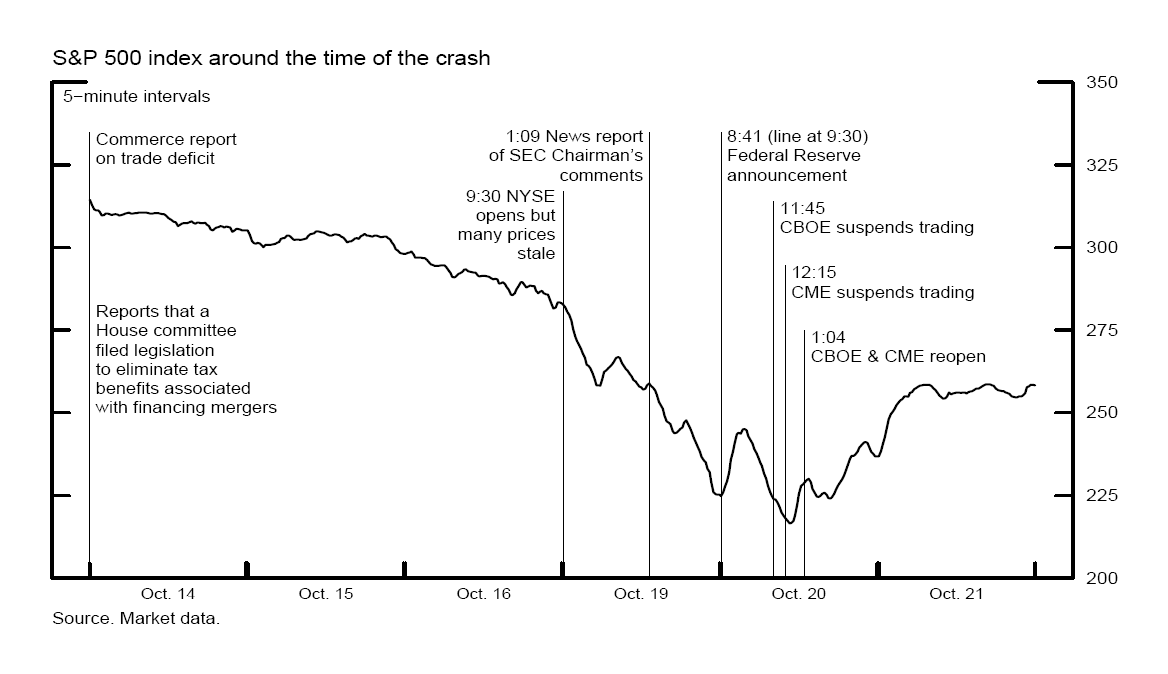
\includegraphics[height=0.38\textheight]{ch5_sp500_1987_fed.png}\\[1mm]
\imgcap{S\&P 500, 14--21 octombrie 1987, date la 5 minute (Federal Reserve)}
\imgcredit{https://commons.wikimedia.org/wiki/File:S\%26P_500_index_around_the_time_of_the_crash.png}{Grafic: M. Carlson, Federal Reserve Board (2006); domeniu public; Wikimedia Commons}
\end{column}
\end{columns}
\end{frame}

\begin{frame}{Septembrie 2008: Lehman Brothers}
\itemsize{\small}
\begin{columns}[T]
\begin{column}{0.60\textwidth}
\begin{itemize}
    \item Lehman Brothers a intrat în faliment pe 15 septembrie 2008; a urmat criza financiară globală
    \begin{itemize}
        \item S\&P 500: $-9{,}5\%$ pe 15 octombrie 2008 și $-9{,}4\%$ pe 1 decembrie 2008
        \item BET: $-13{,}1\%$ pe 7 ianuarie 2009
    \end{itemize}
    \item Pierderile mari au apărut grupat, nu izolat
    \begin{itemize}
        \item volatility clustering (\sfmchlink{https://danpele.github.io/SFM/RO/Cursuri/capitol2_distributii_clasice_fapte_stilizate.pdf}{Capitolul 2}) concentrează extremele în cîteva luni
    \end{itemize}
    \item Un model VaR construit pe distribuția Normală atribuie acestor zile o probabilitate aproape nulă
\end{itemize}
\end{column}
\begin{column}{0.36\textwidth}
\centering

\includegraphics[height=0.46\textheight]{ch5_lehman_2007.jpg}\\[1mm]
\imgcap{Sediul Lehman Brothers, New York, 2007}
\imgcredit{https://commons.wikimedia.org/wiki/File:Lehman_Brothers_Times_Square_by_David_Shankbone.jpg}{Foto: David Shankbone (2007); CC BY-SA 3.0; Wikimedia Commons}
\end{column}
\end{columns}
\end{frame}

\begin{frame}{Martie 2020: crahul COVID-19}
\itemsize{\small}
\begin{columns}[T]
\begin{column}{0.54\textwidth}
\begin{itemize}
    \item Într-o singură săptămînă din martie 2020, trei dintre seriile noastre au înregistrat cea mai mare pierdere zilnică din întreaga perioadă
    \begin{itemize}
        \item S\&P 500: $-12{,}8\%$ pe 16 martie 2020
        \item DAX: $-13{,}1\%$ pe 12 martie 2020
        \item Bitcoin: $-46{,}5\%$ pe 12 martie 2020
    \end{itemize}
    \item Datele acestui capitol
    \begin{itemize}
        \item prețuri de închidere zilnice de la EODHD; S\&P 500 și DAX din 1990, BET din 1997, Bitcoin din 2014
    \end{itemize}
    \item Întrebarea capitolului: cît de des ar trebui să ne așteptăm la o astfel de zi?
\end{itemize}
\end{column}
\begin{column}{0.42\textwidth}
\centering

\includegraphics[height=0.36\textheight]{ch5_fidi_2020.jpg}\\[1mm]
\imgcap{Districtul financiar din New York, pustiu, pe 29 martie 2020}
\imgcredit{https://commons.wikimedia.org/wiki/File:Solitude_(50073346382).jpg}{Foto: Billie Grace Ward (2020); CC BY 2.0; Wikimedia Commons}
\end{column}
\end{columns}
\end{frame}

\begin{frame}{Zilele de crah față de distribuția Normală}
\itemsize{\footnotesize}
\begin{center}
    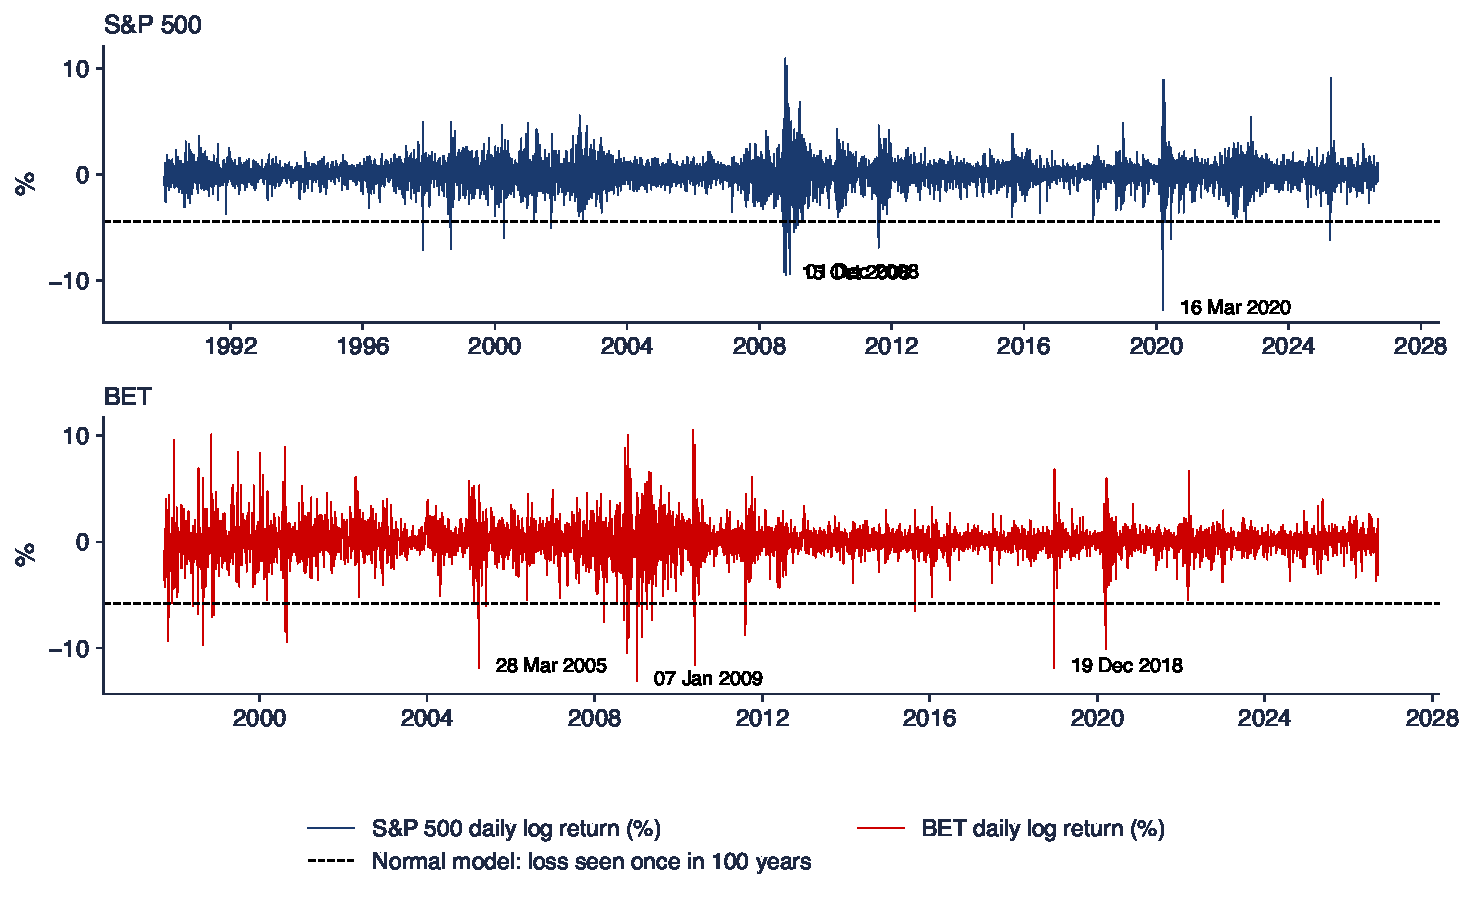
\includegraphics[width=0.97\textwidth,height=0.60\textheight,keepaspectratio]{sfm_ch5_crash_days.pdf}
\end{center}
\vspace{-0.25cm}
\begin{itemize}
    \item Linia punctată: pierderea zilnică depășită o dată la 100 de ani de distribuția Normală ajustată la fiecare serie (S\&P 500: $-4{,}4\%$; BET: $-5{,}8\%$)
    \item Observat: 35 de astfel de zile pentru S\&P 500 din 1990 și 34 pentru BET din 1997
\end{itemize}
\quantlet{SFM\_ch5\_crashes}{\qlurl{SFM_ch5_crashes}}
\end{frame}

\begin{frame}{Cît de rare ar fi cele mai proaste zile sub distribuția Normală?}
\itemsize{\footnotesize}
\begin{center}
\scriptsize
\begin{tabular}{llrrrrr}
\toprule
& cea mai proastă zi & pierdere (\%) & $z$ & distribuția Normală: o dată la (ani) & zile sub $-4\sigma$ & așteptat \\
\midrule
S\&P 500 & 16 martie 2020 & ${-12{,}8}$ & ${-11{,}3}$ & $10^{27}$ & 35 & $0{,}29$ \\
DAX & 12 martie 2020 & ${-13{,}1}$ & ${-9{,}5}$ & $10^{19}$ & 27 & $0{,}29$ \\
BET & 7 ianuarie 2009 & ${-13{,}1}$ & ${-8{,}9}$ & $10^{16}$ & 33 & $0{,}23$ \\
Bitcoin & 12 martie 2020 & ${-46{,}5}$ & ${-13{,}4}$ & $10^{38}$ & 18 & $0{,}14$ \\
\bottomrule
\end{tabular}
\end{center}
\begin{itemize}
    \item $z = (r - \hat\mu)/\hat\sigma$ cu media și abaterea standard a întregului eșantion; o dată la $1/(p \times 252)$ ani (365 de zile pentru Bitcoin)
    \item Timpii de așteptare implicați de distribuția Normală sînt absurzi: mult mai lungi decît istoria oricărei piețe
    \item Pierderi dincolo de $4\sigma$: distribuția Normală prevede mai puțin de o zi pe serie; observăm între 18 și 35
\end{itemize}\quantlet{SFM\_ch5\_crashes}{\qlurl{SFM_ch5_crashes}}
\end{frame}

\begin{frame}{Originile teoriei valorilor extreme}
\itemsize{\small}
\begin{columns}[T]
\begin{column}{0.62\textwidth}
\begin{itemize}
    \item \textbf{EVT} (extreme value theory, teoria valorilor extreme): statistica celor mai mari valori dintr-un eșantion
    \begin{itemize}
        \item folosită întîi pentru inundații, furtuni și rezistența materialelor
        \item \refGumbel: nivelul maxim anual al unui rîu determină înălțimea unui baraj
    \end{itemize}
    \item În finanțe apar aceleași întrebări
    \begin{itemize}
        \item cît de mare este pierderea depășită o dată la 10 ani?
        \item de cît capital este nevoie pentru a acoperi cele mai proaste 1\% dintre zile?
    \end{itemize}
    \item EVT modelează doar coada și lasă datele din coadă să-i determine forma; primele aplicații în finanțe: \refJdV, \refLongin
\end{itemize}
\end{column}
\begin{column}{0.34\textwidth}
\centering
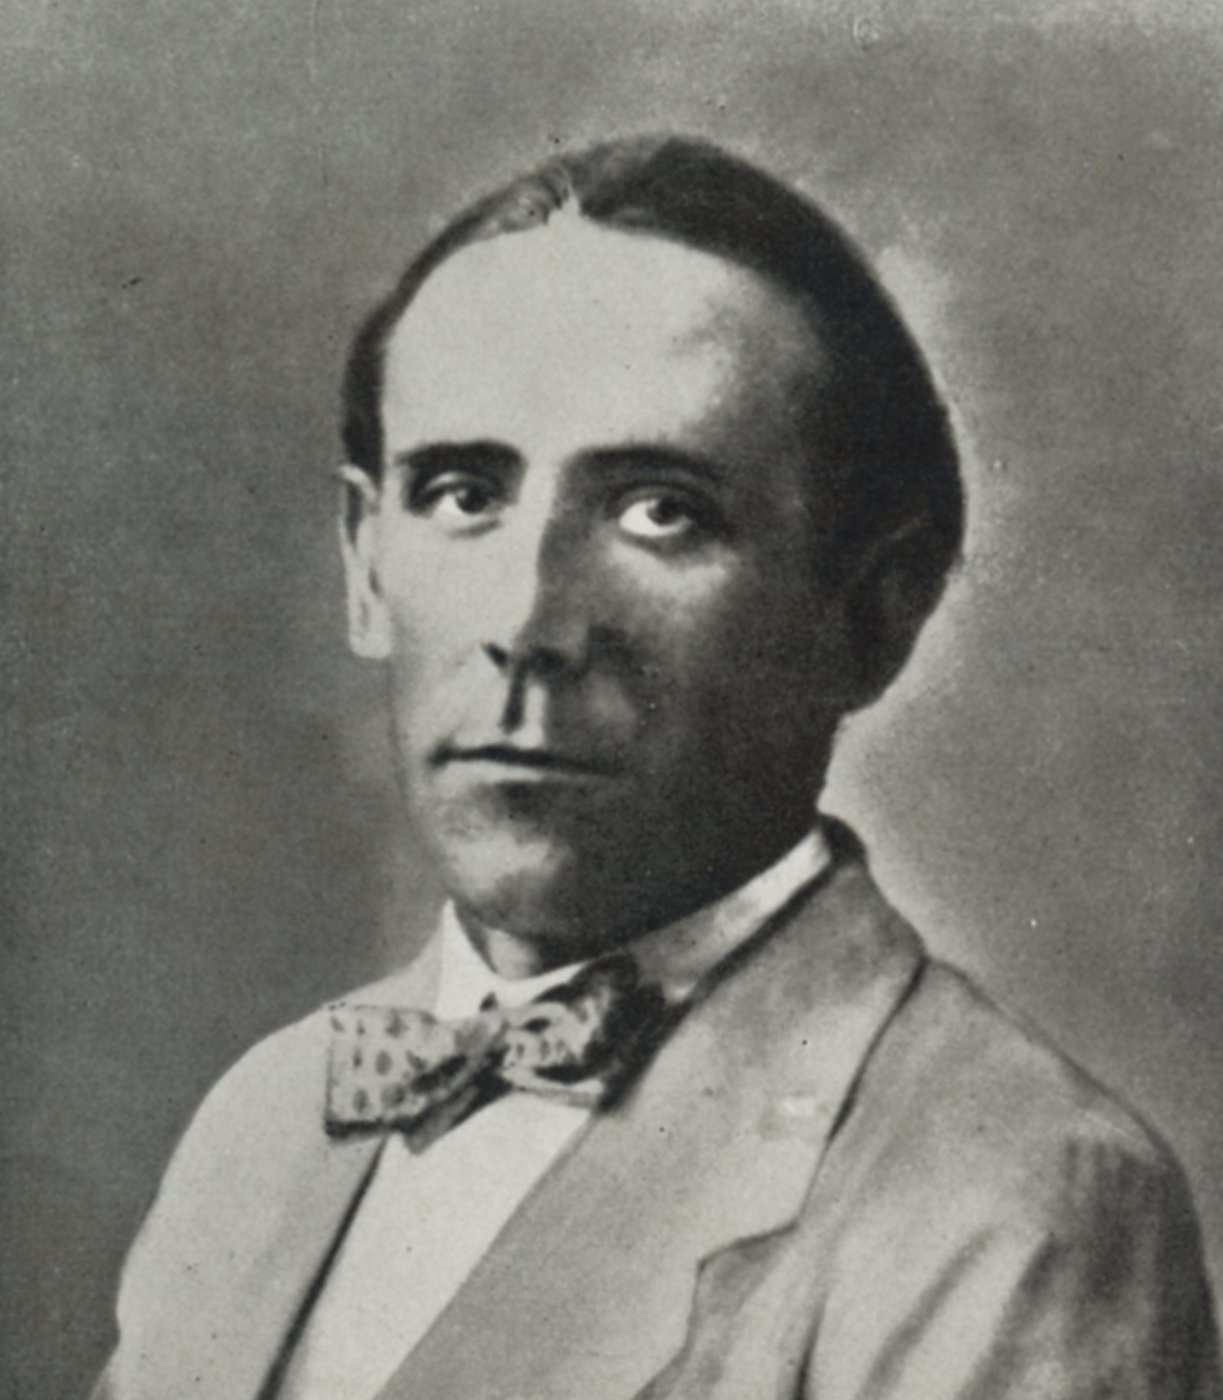
\includegraphics[height=0.44\textheight]{ch5_gumbel_1931.jpg}\\[1mm]
\imgcap{Emil Julius Gumbel (1891--1966)}
\imgcredit{https://commons.wikimedia.org/wiki/File:Emil_Julius_Gumbel.jpg}{Foto: autor necunoscut (c. 1931); domeniu public; Wikimedia Commons}
\end{column}
\end{columns}
\end{frame}

\begin{frame}{De ce contează coada pentru risc}
\itemsize{\small}
\begin{itemize}
    \item \textbf{VaR} (Value at Risk, valoarea expusă la risc) la nivelul $p$: pierderea depășită cu probabilitatea $p$
    \begin{itemize}
        \item $\mathrm{VaR}_p = -q_p(r)$, cu $q_p$ cuantila de ordin $p$ a randamentului; de exemplu VaR 1\%
    \end{itemize}
    \item \textbf{ES} (expected shortfall, pierderea așteptată în coadă) la nivelul $p$: pierderea medie din cele mai proaste $p$ dintre zile
    \begin{itemize}
        \item $\mathrm{ES}_p = -E[r \mid r \le q_p(r)]$; băncile raportează ES 2,5\% conform \refBasel
        \item ES ține seama de întreaga coadă dincolo de VaR și este o măsură de risc coerentă \refAT
    \end{itemize}
    \item Ambele sînt mărimi definite în coadă: un model care descrie greșit coada descrie greșit riscul
    \item \textbf{Întrebare pentru sală}: cu 250 de zile de tranzacționare pe an, de cîți ani de date este nevoie pentru circa 10 zile cu pierderi peste VaR 0,1\%?
    \item \textbf{Răspuns}
    \begin{itemize}
        \item $10 / (0{,}001 \times 250) = 40$ de ani: doar datele istorice nu ajung; EVT extrapolează coada cu un model
    \end{itemize}
\end{itemize}
\end{frame}

\begin{frame}{Recapitulare: de ce contează cozile}
\itemsize{\small}
\begin{itemize}
    \item 1987, 2008, 2020: pierderi zilnice de 10--20\% pentru indici, aproape 50\% pentru Bitcoin
    \item Pentru distribuția Normală, aceste zile nu ar trebui să se întîmple niciodată
    \item VaR și ES sînt mărimi din coadă; puține observații se află atît de departe
    \item EVT: o teorie pentru forma cozii, de la hidrologie la finanțe
\end{itemize}
\end{frame}


%=============================================================================
\section{Cozi groase și variația regulată}
%=============================================================================

\begin{frame}{Cozi subțiri și cozi groase}
\itemsize{\small}
\begin{itemize}
    \item Lucrăm cu pierderile $L = -r$ (în \%): un $L$ mare și pozitiv este o pierdere mare
    \begin{itemize}
        \item \textbf{coada} lui $L$ este descrisă de funcția de supraviețuire $\bar F(x) = P(L > x)$
    \end{itemize}
    \item \textbf{Coadă subțire}: $\bar F(x)$ scade cel puțin la fel de repede ca o exponențială, $e^{-cx}$
    \begin{itemize}
        \item exemple: distribuția Normală ($\bar F(x) \approx e^{-x^2/2}$), distribuția exponențială ($e^{-x}$); toate momentele sînt finite
    \end{itemize}
    \item \textbf{Coadă groasă (de tip putere)}: $\bar F(x)$ scade ca o putere, $x^{-\alpha}$
    \begin{itemize}
        \item exemple: Pareto, Student-t, legile $\alpha$-stabile din \sfmchlink{https://danpele.github.io/SFM/RO/Cursuri/capitol3_distributii_alfa_stabile.pdf}{Capitolul 3}
        \item $\alpha$ este \textbf{indicele de coadă}: cu cît $\alpha$ este mai mic, cu atît coada este mai groasă
    \end{itemize}
\end{itemize}
\end{frame}

\begin{frame}{Legile putere scad mult mai încet}
\itemsize{\footnotesize}
\begin{center}
    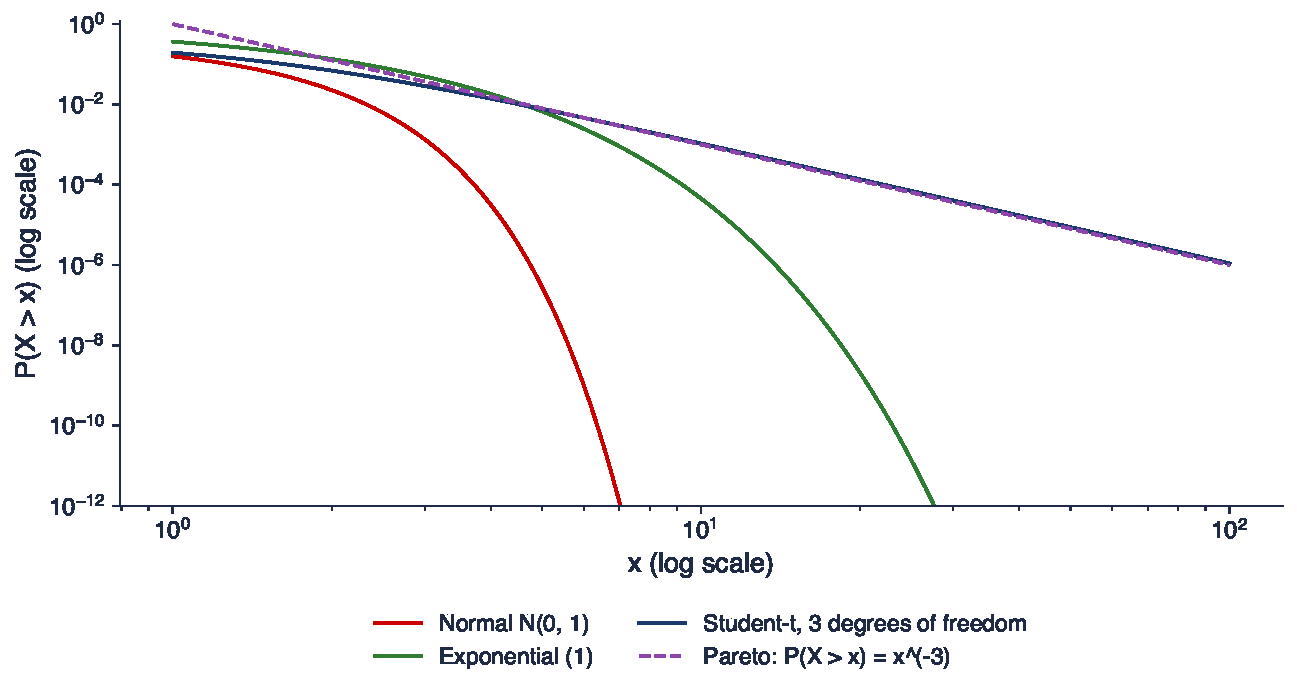
\includegraphics[width=0.97\textwidth,height=0.58\textheight,keepaspectratio]{sfm_ch5_light_heavy.pdf}
\end{center}
\vspace{-0.25cm}
\begin{itemize}
    \item Pe axe log-log, o lege putere este o dreaptă cu panta $-\alpha$; cozile subțiri se curbează în jos și coboară rapid spre zero
    \item $P(X > 10)$: distribuția Normală $7{,}6\times 10^{-24}$, distribuția exponențială $4{,}5\times 10^{-5}$, Student-t cu 3 grade de libertate $1{,}1\times 10^{-3}$
\end{itemize}
\quantlet{SFM\_ch5\_tails\_loglog}{\qlurl{SFM_ch5_tails_loglog}}
\end{frame}

\begin{frame}{Variația regulată și indicele de coadă}
\itemsize{\small}
\begin{itemize}
    \item $L$ are o coadă \textbf{cu variație regulată}, de indice $\alpha > 0$, dacă $\bar F(x) = x^{-\alpha}\ell(x)$
    \begin{itemize}
        \item $\ell$ este \textbf{cu variație lentă}: $\ell(tx)/\ell(x) \to 1$ cînd $x \to \infty$, pentru orice $t > 0$ (de ex.\ o constantă, $\ln x$)
    \end{itemize}
    \item Echivalent: $\dfrac{P(L > tx)}{P(L > x)} \to t^{-\alpha}$ pentru $x$ mare
    \begin{itemize}
        \item dublarea pierderii împarte probabilitatea ei la $2^\alpha$, oricare ar fi nivelul
        \item Student-t cu 3 grade de libertate: $P(X > 20)/P(X > 10) = 0{,}128$, aproape de $2^{-3} = 0{,}125$
    \end{itemize}
    \item Indicii de coadă ai legilor uzuale
    \begin{itemize}
        \item Pareto cu $\bar F(x) = (x/x_0)^{-\alpha}$: indicele $\alpha$; Student-t cu $\nu$ grade de libertate: $\alpha = \nu$
        \item $\alpha$-stabilă cu $\alpha < 2$ (\sfmchlink{https://danpele.github.io/SFM/RO/Cursuri/capitol3_distributii_alfa_stabile.pdf}{Capitolul 3}): același $\alpha$; distribuția Normală: fără coadă de tip putere ($\alpha = \infty$)
    \end{itemize}
\end{itemize}
\end{frame}

\begin{frame}{Indicele de coadă determină momentele care există}
\itemsize{\small}
\begin{itemize}
    \item Pentru o coadă cu variație regulată: $E|L|^m < \infty$ dacă $m < \alpha$ și $E|L|^m = \infty$ dacă $m > \alpha$
    \begin{itemize}
        \item $\alpha \le 1$: nu există media; $\alpha \le 2$: nu există varianța; $\alpha \le 4$: nu există aplatizarea (kurtosis)
    \end{itemize}
    \item „Legea cubică inversă” a randamentelor acțiunilor: $\alpha \approx 3$ \refGopi
    \begin{itemize}
        \item varianța este finită, aplatizarea este infinită: aplatizarea de selecție din \sfmchlink{https://danpele.github.io/SFM/RO/Cursuri/capitol2_distributii_clasice_fapte_stilizate.pdf}{Capitolul 2} nu se stabilizează
    \end{itemize}
    \item Legătura cu \sfmchlink{https://danpele.github.io/SFM/RO/Cursuri/capitol3_distributii_alfa_stabile.pdf}{Capitolul 3}
    \begin{itemize}
        \item parametrul $\alpha$ al legii stabile ($\approx 1{,}5$) se estimează din întreaga distribuție; indicele de coadă de aici folosește doar coada
        \item un indice de coadă în jur de 3 este argumentul împotriva varianței infinite, anunțat în \sfmchlink{https://danpele.github.io/SFM/RO/Cursuri/capitol3_distributii_alfa_stabile.pdf}{Capitolul 3} \refMandelbrot
    \end{itemize}
\end{itemize}
\end{frame}

\begin{frame}{Pierderi reale pe axe log-log}
\itemsize{\footnotesize}
\begin{center}
    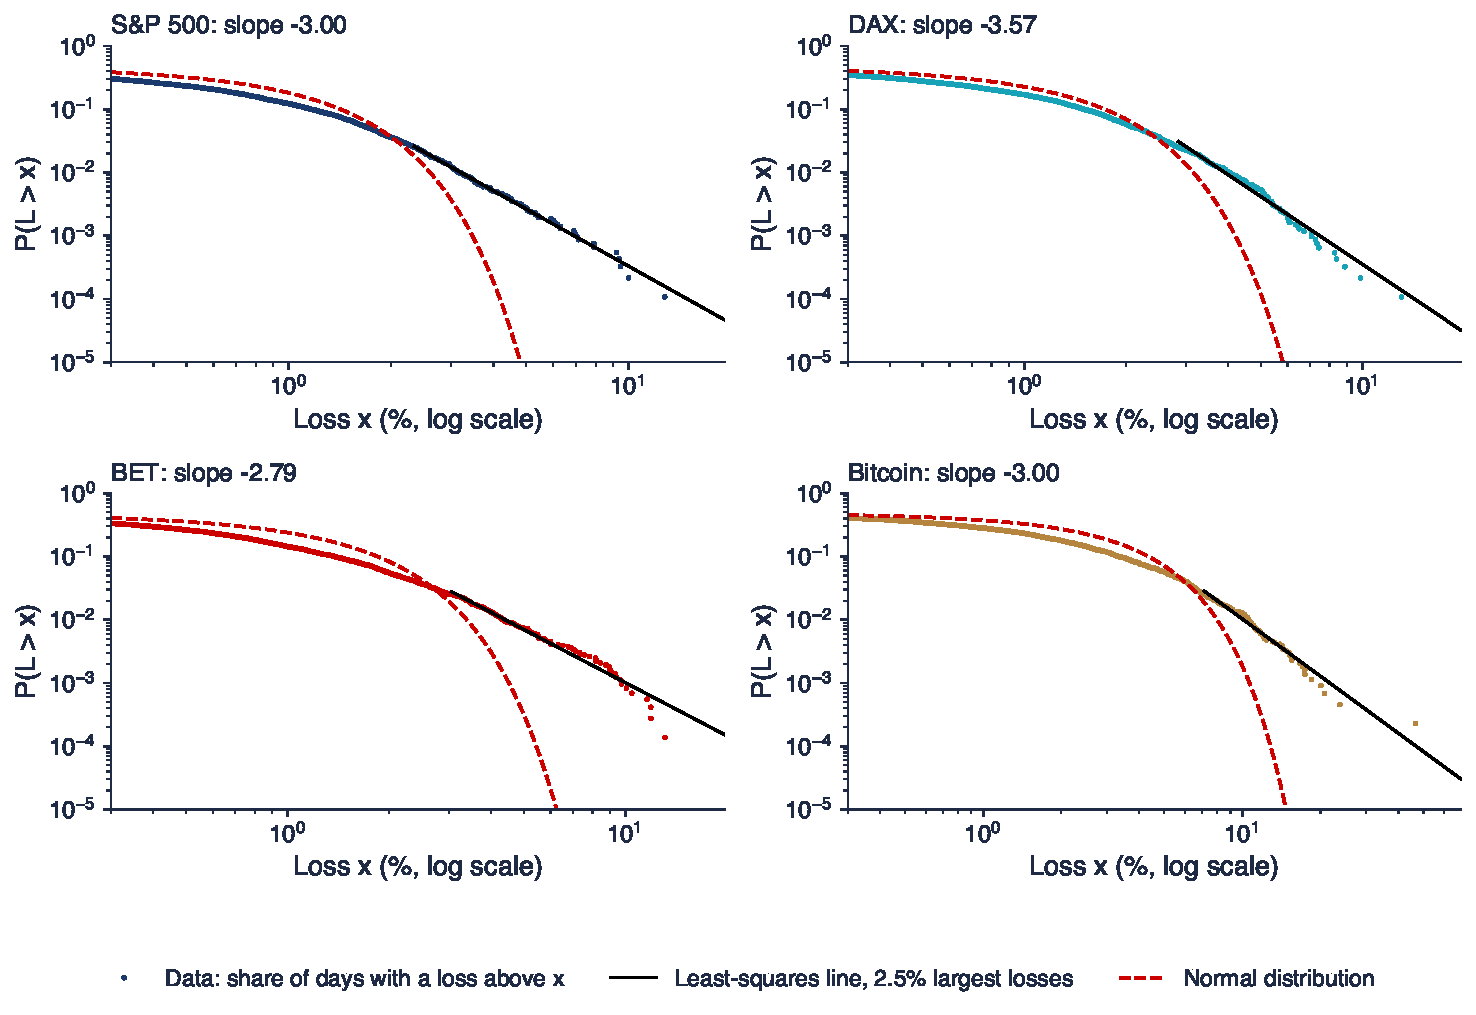
\includegraphics[width=0.97\textwidth,height=0.64\textheight,keepaspectratio]{sfm_ch5_loglog_real.pdf}
\end{center}
\vspace{-0.25cm}
\begin{itemize}
    \item Puncte: proporția zilelor cu o pierdere peste $x$; negru: dreapta celor mai mici pătrate prin cele mai mari 2,5\% dintre pierderi; roșu: distribuția Normală
    \item Pante: S\&P 500 $-3{,}00$, DAX $-3{,}57$, BET $-2{,}79$, Bitcoin $-3{,}00$: drepte, deci cozi de tip putere
\end{itemize}
\quantlet{SFM\_ch5\_tails\_loglog}{\qlurl{SFM_ch5_tails_loglog}}
\end{frame}

\begin{frame}{Interpretarea graficului log-log al cozii}
\itemsize{\small}
\begin{itemize}
    \item Dacă $\bar F(x) \approx C x^{-\alpha}$, atunci $\ln \bar F(x) \approx \ln C - \alpha \ln x$: o dreaptă cu panta $-\alpha$
    \begin{itemize}
        \item \textbf{estimatorul celor mai mici pătrate}: regresia lui $\ln(i/n)$ pe $\ln L_{(i)}$ pentru cele mai mari $k$ pierderi $L_{(1)} \ge \dots \ge L_{(k)}$
        \item $L_{(i)}$ este a $i$-a cea mai mare pierdere, o \textbf{statistică de ordine}
    \end{itemize}
    \item Corpul distribuției (pierderile mici) se depărtează de dreaptă: legea putere este valabilă doar în coadă
    \item Coada distribuției Normale coboară sub date încă de la pierderi de 3--4\%, pentru indici
    \item Panta celor mai mici pătrate este simplă, dar punctele folosite nu sînt independente; estimatorul Hill este instrumentul standard
\end{itemize}\quantlet{SFM\_ch5\_tails\_loglog}{\qlurl{SFM_ch5_tails_loglog}}
\end{frame}

\begin{frame}{Exemplu lucrat: o coadă Pareto}
\itemsize{\small}
\begin{itemize}
    \item Pierderile zilnice au o coadă Pareto cu $\alpha = 3$ și $P(L > 3\%) = 1\%$
    \begin{itemize}
        \item $P(L > x) = 1\% \times (x/3)^{-3}$ pentru $x \ge 3\%$
    \end{itemize}
    \item Pierdere peste 6\%: $1\% \times 2^{-3} = 0{,}125\%$; peste 9\%: $1\% \times 3^{-3} = 0{,}037\%$
    \begin{itemize}
        \item dublarea pierderii împarte probabilitatea la $2^3 = 8$
    \end{itemize}
    \item \textbf{Ce credeți?} Ce pierdere este depășită cu probabilitatea 0,1\% (VaR 0,1\%)?
    \item \textbf{Răspuns}
    \begin{itemize}
        \item rezolvăm $1\% \times (x/3)^{-3} = 0{,}1\%$: $x = 3 \times 10^{1/3} = 3 \times 2{,}15 = 6{,}46\%$
        \item o probabilitate de zece ori mai mică crește pierderea doar cu factorul $10^{1/\alpha}$
    \end{itemize}
\end{itemize}
\end{frame}

\begin{frame}{Recapitulare: cozi groase}
\itemsize{\small}
\begin{itemize}
    \item Coadă groasă: $P(L > x) = x^{-\alpha}\ell(x)$, o dreaptă pe axe log-log
    \item Indicele de coadă $\alpha$ determină momentele care există: cele de ordin mai mic decît $\alpha$
    \item Pierderile zilnice ale indicilor: pante în jur de 3, legea cubică inversă
    \item Lege putere: VaR crește doar de $10^{1/\alpha}$ ori cînd probabilitatea scade de zece ori
\end{itemize}
\end{frame}


%=============================================================================
\section{Estimatorul Hill}
%=============================================================================

\begin{frame}{Estimatorul Hill}
\itemsize{\small}
\begin{itemize}
    \item Ordonăm pierderile: $L_{(1)} \ge L_{(2)} \ge \dots \ge L_{(n)}$; păstrăm cele mai mari $k$
    \begin{itemize}
        \item \textbf{Estimatorul Hill} \refHill: $\hat\alpha_k = \Big[\dfrac{1}{k}\sum_{i=1}^{k}\ln\dfrac{L_{(i)}}{L_{(k+1)}}\Big]^{-1}$
        \item pragul este a $(k+1)$-a cea mai mare pierdere, $u = L_{(k+1)}$
    \end{itemize}
    \item De ce funcționează: dacă $P(L > x \mid L > u) = (x/u)^{-\alpha}$ (Pareto peste $u$), atunci $\ln(L/u)$, condiționat de $L > u$, are distribuție exponențială cu media $1/\alpha$
    \begin{itemize}
        \item media celor $k$ excese logaritmice estimează $1/\alpha$; inversa ei estimează $\alpha$
        \item Hill $=$ estimatorul de verosimilitate maximă al unei cozi Pareto peste $u$
    \end{itemize}
    \item Portat din Quantlet-ul SFE SFElshill (estimatorii celor mai mici pătrate și Hill ai indicelui de coadă) \refFHH
\end{itemize}
\end{frame}

\begin{frame}{Exemplu lucrat: Hill pe șase pierderi}
\itemsize{\small}
\begin{itemize}
    \item Cele mai mari șase pierderi zilnice (\%): $9{,}5$; $7{,}2$; $6{,}1$; $5{,}4$; $4{,}8$; $4{,}0$; luăm $k = 5$, deci $L_{(6)} = 4{,}0$
    \item Excesele logaritmice $\ln(L_{(i)}/4{,}0)$
    \begin{itemize}
        \item $0{,}865$; $0{,}588$; $0{,}422$; $0{,}300$; $0{,}182$; media $0{,}471$
    \end{itemize}
    \item $\hat\alpha_5 = 1/0{,}471 = 2{,}12$
    \item Eroarea standard în ipoteza de independență: $\mathrm{SE}(\hat\alpha) \approx \hat\alpha/\sqrt{k} = 0{,}95$
    \begin{itemize}
        \item cu $k = 5$, estimarea este foarte imprecisă: aplicațiile reale folosesc sute de pierderi
    \end{itemize}
\end{itemize}
\end{frame}

\begin{frame}{Alegerea lui $k$: graficul Hill}
\itemsize{\small}
\begin{itemize}
    \item \textbf{$k$ mic}: doar coada îndepărtată, puține puncte: varianță mare
    \item \textbf{$k$ mare}: intră corpul distribuției, unde legea putere nu mai este valabilă: deplasare (bias)
    \item \textbf{Graficul Hill (Hill plot)}: $\hat\alpha_k$ în funcție de $k$; căutăm o zonă în care graficul este aproximativ orizontal \refDRH
    \begin{itemize}
        \item aici $k$ apare ca proporție din eșantion, $k/n$ între 0,5\% și 10\%
    \end{itemize}
    \item Fixăm regula înainte de a vedea rezultatul: aici $k = 2{,}5\%$ din $n$
    \begin{itemize}
        \item și raportăm estimările pentru $k = 1\%$ și $5\%$ din $n$, ca verificare
    \end{itemize}
\end{itemize}
\end{frame}

\begin{frame}{Grafice Hill ale pierderilor zilnice}
\itemsize{\footnotesize}
\begin{center}
    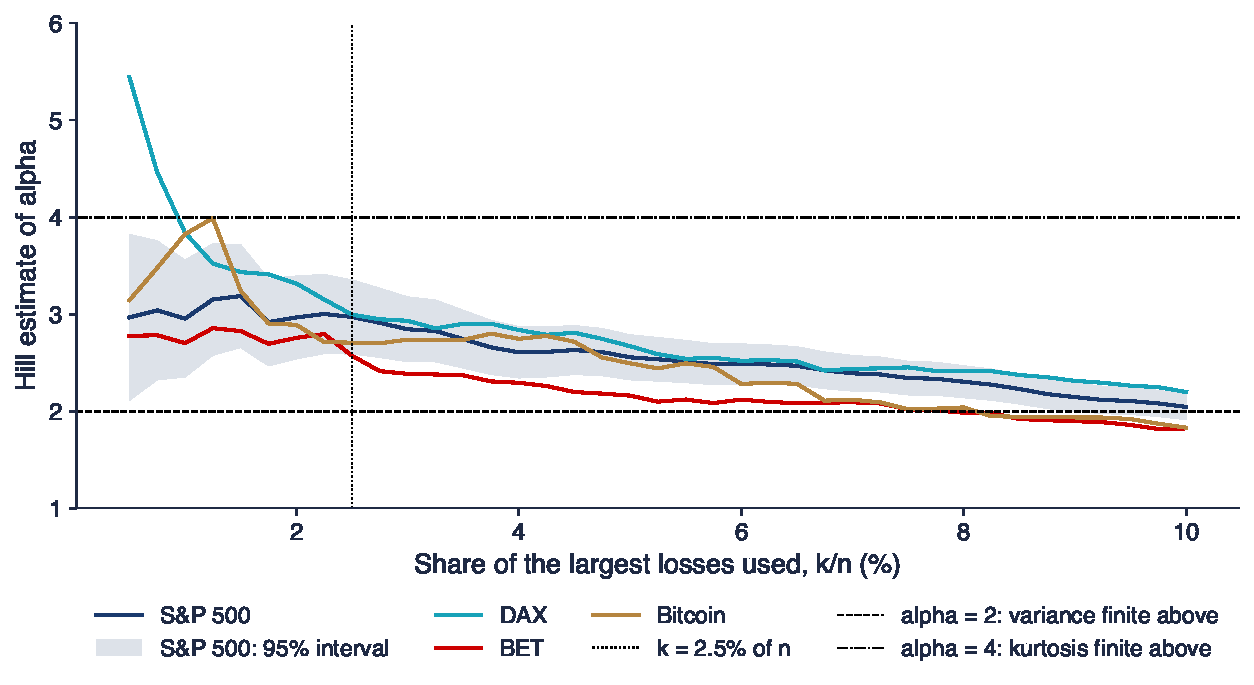
\includegraphics[width=0.97\textwidth,height=0.60\textheight,keepaspectratio]{sfm_ch5_hill_plot.pdf}
\end{center}
\vspace{-0.25cm}
\begin{itemize}
    \item Între 1\% și 5\% din $n$, curbele sînt aproximativ orizontale, în mare parte între 2 și 3,5; banda: intervalul de 95\% pentru S\&P 500
    \item Peste 5\%, estimările coboară: corpul distribuției introduce o deplasare în $\hat\alpha$
\end{itemize}
\quantlet{SFM\_ch5\_hill}{\qlurl{SFM_ch5_hill}}
\end{frame}

\begin{frame}{Inferența pentru estimatorul Hill}
\itemsize{\small}
\begin{itemize}
    \item Pentru date i.i.d.\ cu coadă de tip Pareto: $\sqrt{k}\,(\hat\alpha_k - \alpha) \to N(0, \alpha^2)$, pentru $k \to \infty$, $k/n \to 0$
    \begin{itemize}
        \item i.i.d.: independente și identic distribuite; $\mathrm{SE} = \hat\alpha/\sqrt{k}$, CI de 95\% $\hat\alpha(1 \pm 1{,}96/\sqrt{k})$
    \end{itemize}
    \item Randamentele nu sînt independente: pierderile mari apar grupat (volatility clustering)
    \begin{itemize}
        \item \textbf{bootstrap pe blocuri mobile}: reeșantionăm blocuri de 20 de zile consecutive, recalculăm $\hat\alpha$ și calculăm abaterea standard a estimărilor
        \item blocurile păstrează episoadele grupate, deci eroarea standard ține seama de dependență
    \end{itemize}
    \item Aceeași regulă pentru fiecare serie: $k = 2{,}5\%$ din $n$, 500 de eșantioane bootstrap
\end{itemize}
\end{frame}

\begin{frame}{Estimări Hill pentru patru piețe}
\itemsize{\footnotesize}
\begin{center}
\scriptsize
\begin{tabular}{lrrrrrrrr}
\toprule
& $n$ & $k$ & $\hat\alpha$ & CI 95\% & SE i.i.d. & SE blocuri & $k = 1\%$ / $5\%$ & cîștiguri \\
\midrule
S\&P 500 & 9\,240 & 231 & $2{,}97$ & $[2{,}59; 3{,}35]$ & $0{,}20$ & $0{,}30$ & $2{,}95$ / $2{,}56$ & $2{,}96$ \\
DAX & 9\,288 & 232 & $3{,}00$ & $[2{,}61; 3{,}38]$ & $0{,}20$ & $0{,}20$ & $3{,}84$ / $2{,}67$ & $3{,}22$ \\
BET & 7\,243 & 181 & $2{,}57$ & $[2{,}20; 2{,}95]$ & $0{,}19$ & $0{,}23$ & $2{,}70$ / $2{,}16$ & $2{,}82$ \\
Bitcoin & 4\,384 & 109 & $2{,}71$ & $[2{,}20; 3{,}21]$ & $0{,}26$ & $0{,}23$ & $3{,}83$ / $2{,}49$ & $3{,}37$ \\
\bottomrule
\end{tabular}
\end{center}
\begin{itemize}
    \item Pierderi: $\hat\alpha$ între $2{,}57$ și $3{,}00$; intervalele exclud 2 (varianță finită) și sînt sub 4 (aplatizare infinită)
    \item SE din bootstrap pe blocuri este apropiată aici de cea i.i.d.; estimările variază cu $k$ cu mai mult de o SE
    \item Ultima coloană: indicele Hill al cîștigurilor ($r_t > 0$), același $k$
\end{itemize}\quantlet{SFM\_ch5\_hill}{\qlurl{SFM_ch5_hill}}
\end{frame}

\begin{frame}{De la indicele de coadă la o cuantilă}
\itemsize{\small}
\begin{itemize}
    \item \textbf{Cuantila Hill (Weissman)} \refWeissman: $\hat x_p = L_{(k+1)}\Big(\dfrac{k}{n p}\Big)^{1/\hat\alpha}$
    \begin{itemize}
        \item pierderea depășită cu probabilitatea $p$, extrapolată de la prag cu legea putere; Quantlet-ul SFE SFEhillquantile
    \end{itemize}
    \item \textbf{Exemplu lucrat}, S\&P 500, VaR 0,1\%: $n = 9\,240$, $k = 231$, $L_{(k+1)} = 2{,}34\%$, $\hat\alpha = 2{,}97$
    \begin{itemize}
        \item $k/(np) = 231/9{,}24 = 25{,}0$; $25{,}0^{1/2{,}97} = 2{,}95$
        \item $\hat x_{0{,}001} = 2{,}34 \times 2{,}95 = 6{,}92\%$; cuantila empirică de 0,1\%: $6{,}94\%$
    \end{itemize}
    \item Extrapolarea este doar atît de bună cît este $\hat\alpha$: o eroare de o SE în $\hat\alpha$ modifică vizibil $\hat x_p$
\end{itemize}\quantlet{SFM\_ch5\_hill}{\qlurl{SFM_ch5_hill}}
\end{frame}

\begin{frame}{Patru acțiuni de la Bursa de Valori București}
\itemsize{\footnotesize}
\begin{columns}[T]
\begin{column}{0.60\textwidth}
\begin{center}
\scriptsize
\begin{tabular}{lrrrrr}
\toprule
& $n$ & $\hat\alpha$ & CI 95\% & SE blocuri & cîștiguri \\
\midrule
OMV Petrom (SNP) & 3\,815 & $2{,}96$ & $[2{,}36; 3{,}56]$ & $0{,}39$ & $3{,}71$ \\
BRD & 3\,771 & $3{,}22$ & $[2{,}57; 3{,}87]$ & $0{,}33$ & $3{,}77$ \\
Banca Transilvania (TLV) & 3\,788 & $2{,}49$ & $[1{,}98; 2{,}99]$ & $0{,}28$ & $3{,}55$ \\
Transgaz (TGN) & 3\,725 & $3{,}02$ & $[2{,}41; 3{,}64]$ & $0{,}31$ & $3{,}56$ \\
\bottomrule
\end{tabular}
\end{center}
\begin{itemize}
    \item Randamente logaritmice zilnice, calculate din prețul ajustat, din 2010; $k = 2{,}5\%$ din $n$
    \item TLV: zilele de 30--31 mai 2016 sînt eliminate, din cauza unei ajustări înregistrate cu o zi întîrziere (\sfmchlink{https://danpele.github.io/SFM/RO/Cursuri/capitol2_distributii_clasice_fapte_stilizate.pdf}{Capitolul 2})
    \item Toate cele patru acțiuni: $\hat\alpha$ între $2{,}49$ și $3{,}22$, ca la indici; pierderile au cozi mai groase decît cîștigurile
\end{itemize}
\end{column}
\begin{column}{0.36\textwidth}
\centering
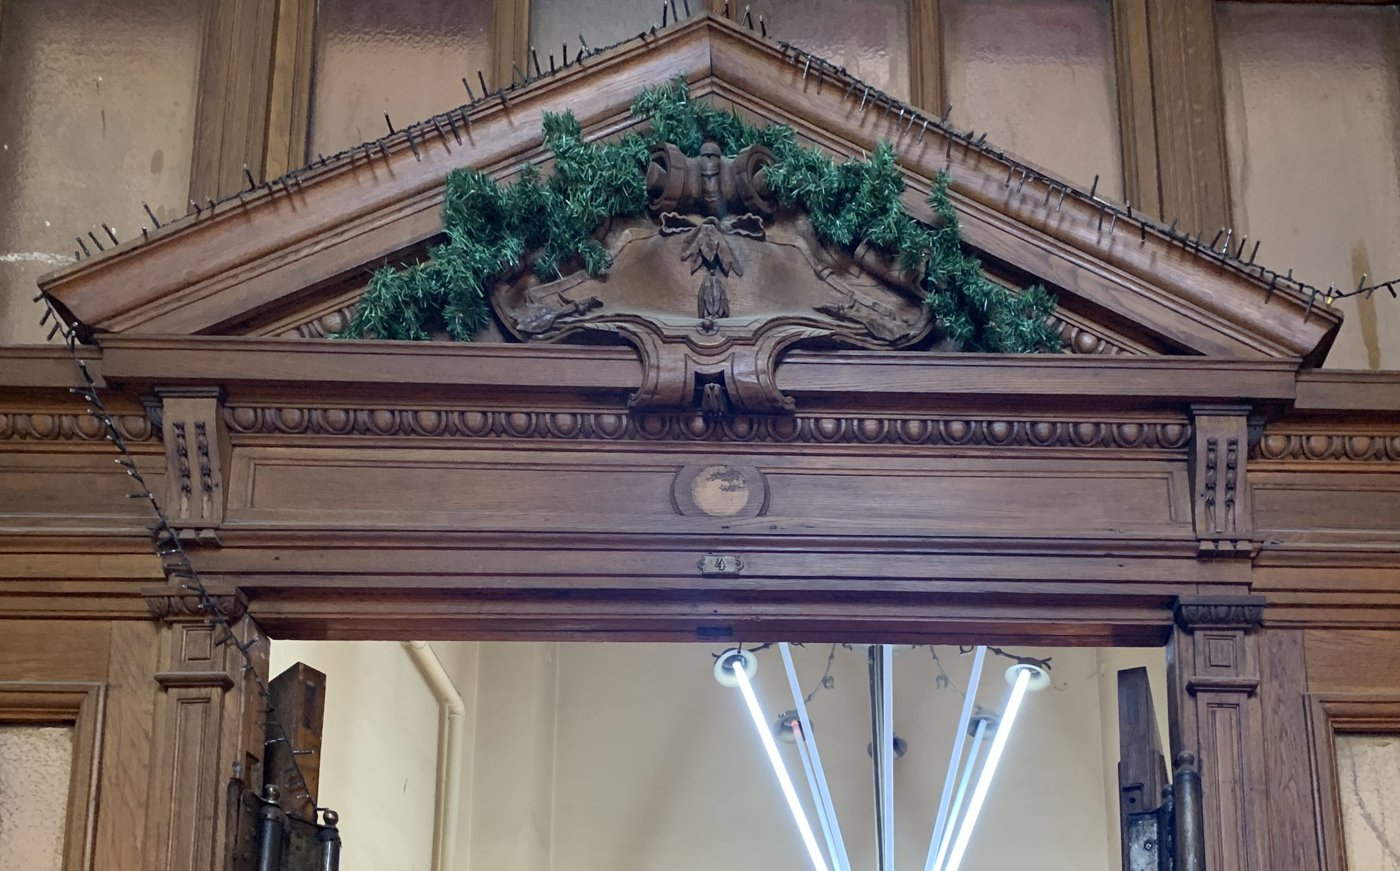
\includegraphics[height=0.32\textheight]{ch5_bvb_palace_2019.jpg}\\[1mm]
\imgcap{Palatul Bursei, București}
\imgcredit{https://commons.wikimedia.org/wiki/File:Stock_Exchange_Palace_(Bucharest).jpg}{Foto: Neoclassicism Enthusiast (2019); CC BY-SA 4.0; Wikimedia Commons}
\end{column}
\end{columns}\quantlet{SFM\_ch5\_hill}{\qlurl{SFM_ch5_hill}}
\end{frame}

\begin{frame}{Grafice Hill pentru acțiunile BVB}
\itemsize{\footnotesize}
\begin{center}
    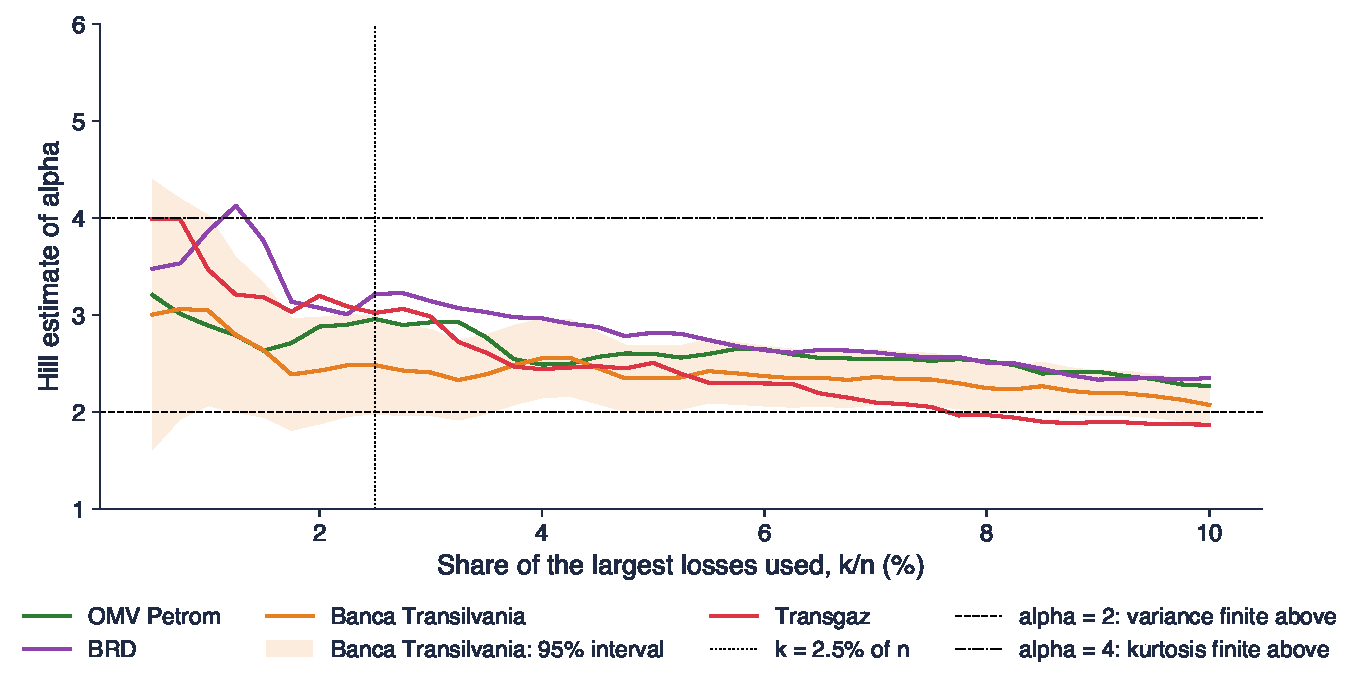
\includegraphics[width=0.97\textwidth,height=0.58\textheight,keepaspectratio]{sfm_ch5_hill_bvb.pdf}
\end{center}
\vspace{-0.25cm}
\begin{itemize}
    \item Eșantioane mai scurte ($n \approx 3\,800$): benzi mai largi (afișată pentru TLV) și mai multe oscilații la $k$ mic
    \item Nicio acțiune nu are $\hat\alpha$ sub 2 în zona plată: varianțele sînt finite
\end{itemize}
\quantlet{SFM\_ch5\_hill}{\qlurl{SFM_ch5_hill}}
\end{frame}

\begin{frame}{Recapitulare: estimatorul Hill}
\itemsize{\small}
\begin{itemize}
    \item $\hat\alpha_k = [\frac1k\sum_{i \le k}\ln(L_{(i)}/L_{(k+1)})]^{-1}$, estimatorul ML al unei cozi Pareto
    \item Alegeți $k$ acolo unde graficul Hill este plat; fixați regula dinainte
    \item SE $\approx \hat\alpha/\sqrt{k}$; bootstrap pe blocuri pentru randamente dependente
    \item Indici și acțiuni BVB: $\hat\alpha$ între $2{,}49$ și $3{,}22$, varianță finită, aplatizare infinită
\end{itemize}
\end{frame}


%=============================================================================
\section{Funcția mean excess}
%=============================================================================

\begin{frame}{Funcția mean excess}
\itemsize{\small}
\begin{itemize}
    \item \textbf{Funcția mean excess} (excesul mediu): $e(u) = E[L - u \mid L > u]$, pierderea medie peste $u$, știind că $u$ este depășit
    \begin{itemize}
        \item versiunea empirică: media lui $L_i - u$ pentru pierderile cu $L_i > u$
    \end{itemize}
    \item Forma ei arată tipul de coadă
    \begin{itemize}
        \item distribuția exponențială: $e(u)$ constantă (lipsa memoriei)
        \item Pareto cu $\alpha > 1$: $e(u) = u/(\alpha - 1)$, o dreaptă crescătoare
        \item distribuția Normală: $e(u)$ scade spre 0 (aproximativ $1/u$ pentru distribuția Normală standard)
    \end{itemize}
    \item \textbf{Exemplu}: coadă Pareto cu $\alpha = 3$: $e(u) = u/2$
    \begin{itemize}
        \item peste o pierdere de 2\%, pierderea suplimentară medie este $1{,}0\%$; peste 4\% este $2{,}0\%$: cu cît pragul este mai mare, cu atît excesul mediu este mai mare
    \end{itemize}
\end{itemize}
\end{frame}

\begin{frame}{Mean excess empiric al pierderilor zilnice}
\itemsize{\footnotesize}
\begin{center}
    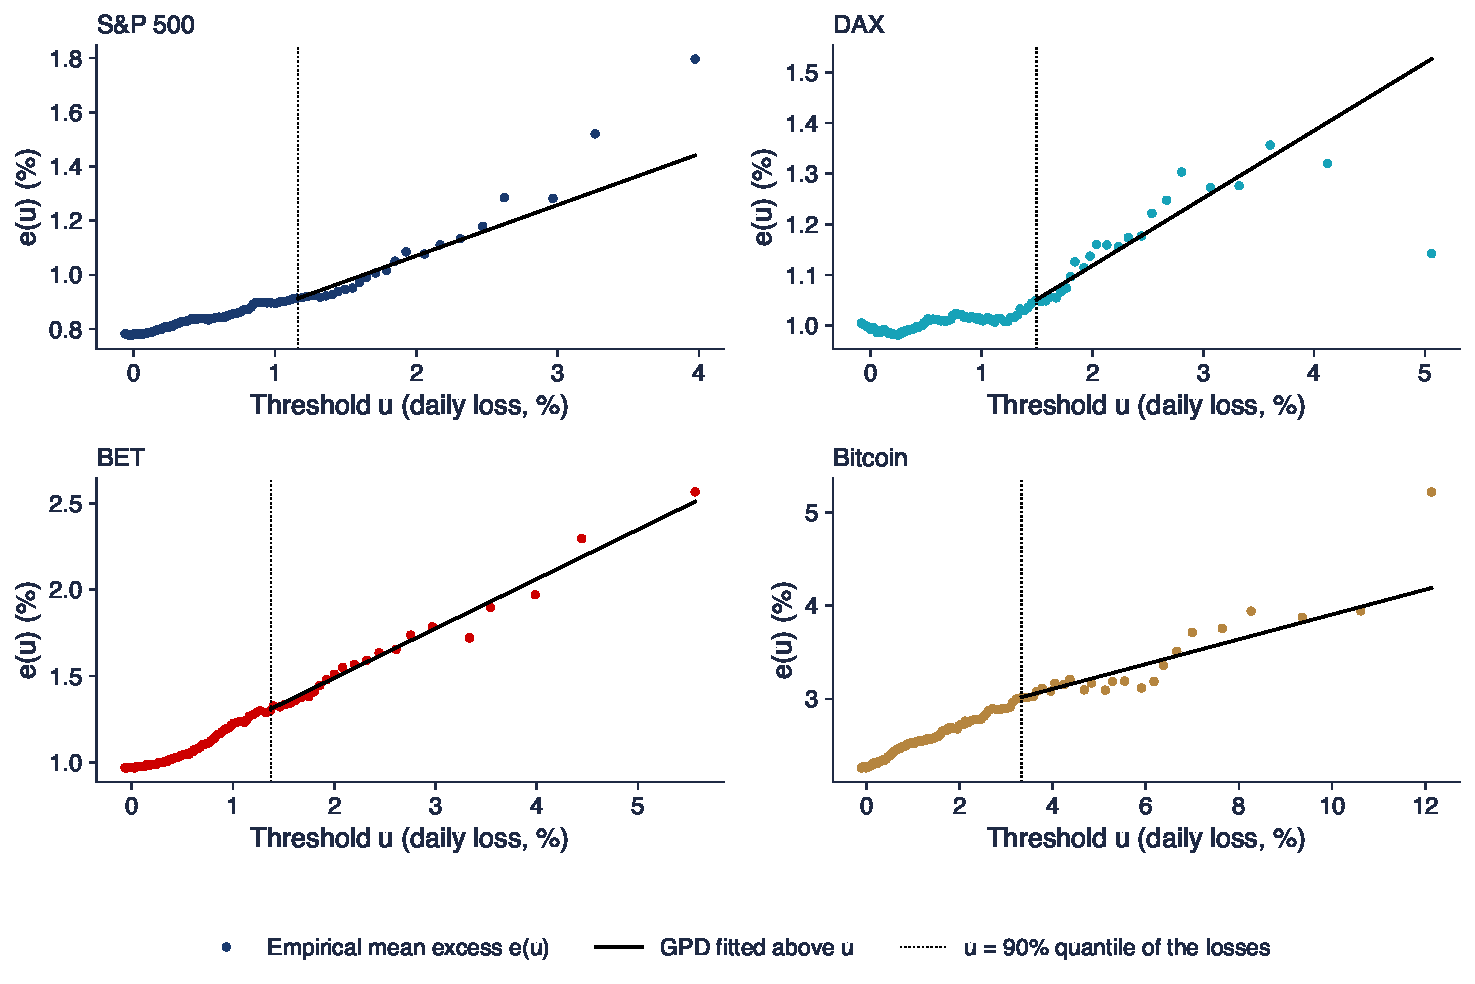
\includegraphics[width=0.97\textwidth,height=0.62\textheight,keepaspectratio]{sfm_ch5_mean_excess.pdf}
\end{center}
\vspace{-0.25cm}
\begin{itemize}
    \item Toate cele patru funcții cresc peste cuantila de 90\% $u$ (punctat): o coadă groasă, de tip Pareto; negru: dreapta implicată de GPD ajustată peste $u$
    \item Ultimele puncte se bazează pe foarte puține pierderi și sînt instabile: nu le interpretați literal
\end{itemize}
\quantlet{SFM\_ch5\_mean\_excess}{\qlurl{SFM_ch5_mean_excess}}
\end{frame}

\begin{frame}{Interpretarea graficului mean excess}
\itemsize{\small}
\begin{itemize}
    \item Căutăm pragul peste care $e(u)$ devine aproximativ o dreaptă
    \begin{itemize}
        \item o dreaptă crescătoare înseamnă o coadă groasă; panta ei dă o primă idee despre forma cozii
    \end{itemize}
    \item La cuantila de 90\%: $e(u)$ este $0{,}92\%$ pentru S\&P 500 ($u = 1{,}16\%$) și $1{,}30\%$ pentru BET ($u = 1{,}38\%$)
    \begin{itemize}
        \item într-o zi cu o pierdere peste $u$, excesul peste $u$ este, în medie, aproximativ egal cu $u$
    \end{itemize}
    \item Funcția mean excess este unul dintre instrumentele pentru alegerea pragului în metoda peaks over threshold (Secțiunea 6)
    \item Portată din Quantlet-ul SFE SFEMeanExcessFun
\end{itemize}\quantlet{SFM\_ch5\_mean\_excess}{\qlurl{SFM_ch5_mean_excess}}
\end{frame}


%=============================================================================
\section{Block maxima și distribuția GEV}
%=============================================================================

\begin{frame}{Maxime pe blocuri (block maxima)}
\itemsize{\small}
\begin{columns}[T]
\begin{column}{0.62\textwidth}
\begin{itemize}
    \item Împărțim pierderile în blocuri de aceeași lungime și păstrăm cea mai mare pierdere din fiecare bloc
    \begin{itemize}
        \item $M_n = \max(L_1, \dots, L_n)$, aici cea mai mare pierdere zilnică din fiecare lună calendaristică ($n \approx 21$)
    \end{itemize}
    \item Întrebarea: care este legea lui $M_n$ pentru $n$ mare?
    \begin{itemize}
        \item analogul teoremei limită centrale, pentru maxime în loc de sume
    \end{itemize}
    \item \refFT\ au găsit cele trei legi limită posibile, studiind cel mai mare element al unui eșantion
\end{itemize}
\end{column}
\begin{column}{0.34\textwidth}
\centering

\includegraphics[height=0.42\textheight]{ch5_fisher_1913.jpg}\\[1mm]
\imgcap{Ronald A. Fisher (1890--1962), în 1913}
\imgcredit{https://commons.wikimedia.org/wiki/File:Youngronaldfisher2.JPG}{Foto: autor necunoscut (1913); domeniu public; Wikimedia Commons}
\end{column}
\end{columns}
\end{frame}

\begin{frame}{Teorema Fisher--Tippett--Gnedenko}
\itemsize{\small}
\begin{itemize}
    \item $L_1, L_2, \dots$ i.i.d. Dacă există constante $a_n > 0$, $b_n$ astfel încît $P\Big(\dfrac{M_n - b_n}{a_n} \le x\Big) \to H(x)$, nedegenerată,
    \begin{itemize}
        \item atunci $H$ este o distribuție \textbf{GEV} (generalised extreme value, distribuția generalizată a valorilor extreme) \refFT, \refGnedenko
    \end{itemize}
    \item \textbf{GEV} cu forma $\xi$, locația $\mu$, scala $\sigma > 0$ (forma unificată a lui \refJenkinson)
    \begin{itemize}
        \item $H(x) = \exp\Big\{-\Big[1 + \xi\,\dfrac{x - \mu}{\sigma}\Big]^{-1/\xi}\Big\}$ pentru $1 + \xi(x - \mu)/\sigma > 0$
        \item $\xi = 0$: $H(x) = \exp\{-e^{-(x - \mu)/\sigma}\}$, limita pentru $\xi \to 0$
    \end{itemize}
    \item Oricare ar fi legea pierderilor, maximul normalizat are o singură familie de limite posibile
\end{itemize}
\end{frame}

\begin{frame}{Trei tipuri într-o singură familie}
\itemsize{\small}
\begin{columns}[T]
\begin{column}{0.64\textwidth}
\begin{itemize}
    \item \textbf{Fréchet} ($\xi > 0$): coadă groasă, $1 - H(x) \sim x^{-1/\xi}$
    \begin{itemize}
        \item indicele de coadă $\alpha = 1/\xi$; cazul pierderilor financiare
    \end{itemize}
    \item \textbf{Gumbel} ($\xi = 0$): coadă subțire, exponențială
    \begin{itemize}
        \item maximele variabilelor cu distribuție Normală, lognormală sau exponențială
    \end{itemize}
    \item \textbf{Weibull} ($\xi < 0$): un capăt superior finit $\mu - \sigma/\xi$
    \begin{itemize}
        \item maximele variabilelor mărginite (uniformă, Beta)
    \end{itemize}
    \item Mulțimea legilor ale căror maxime converg către un $H$ dat este \textbf{domeniul de atracție al maximului} său
\end{itemize}
\end{column}
\begin{column}{0.32\textwidth}
\centering

\includegraphics[height=0.40\textheight]{ch5_frechet.jpg}\\[1mm]
\imgcap{Maurice Fréchet (1878--1973)}
\imgcredit{https://commons.wikimedia.org/wiki/File:Frechet.jpeg}{Foto: autor necunoscut; domeniu public; Wikimedia Commons}
\end{column}
\end{columns}
\end{frame}

\begin{frame}{Cele trei legi ale valorilor extreme}
\itemsize{\footnotesize}
\begin{center}
    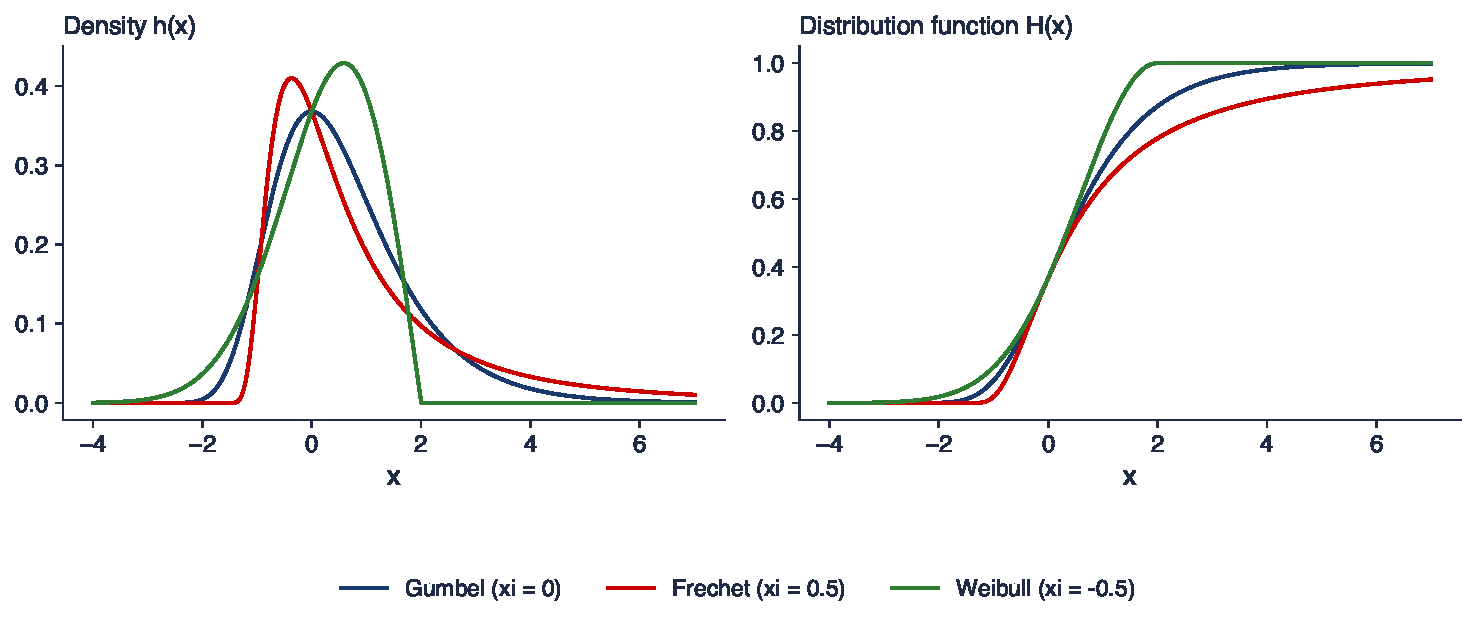
\includegraphics[width=0.97\textwidth,height=0.56\textheight,keepaspectratio]{sfm_ch5_gev_types.pdf}
\end{center}
\vspace{-0.25cm}
\begin{itemize}
    \item Parametri de locație și de scală standard ($\mu = 0$, $\sigma = 1$): Fréchet are cea mai lungă coadă dreaptă, Weibull se oprește la $x = 2$
    \item Portat din Quantlet-ul SFE SFEevt1
\end{itemize}
\quantlet{SFM\_ch5\_gev\_block\_maxima}{\qlurl{SFM_ch5_gev_block_maxima}}
\end{frame}

\begin{frame}{Teorema într-o simulare}
\itemsize{\footnotesize}
\begin{center}
    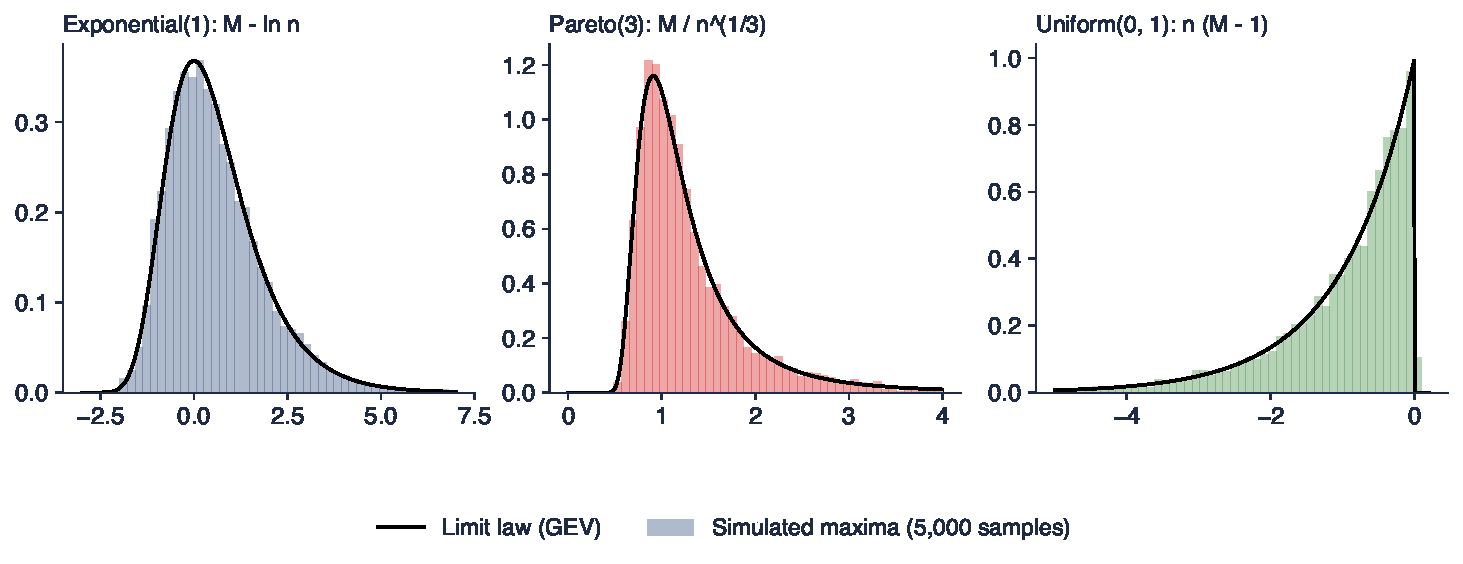
\includegraphics[width=0.97\textwidth,height=0.44\textheight,keepaspectratio]{sfm_ch5_maxima_sim.pdf}
\end{center}
\vspace{-0.25cm}
\begin{itemize}
    \item 5\,000 de eșantioane de $n = 250$; maximele exponențiale minus $\ln n$ $\to$ Gumbel; maximele Pareto(3) împărțite la $n^{1/3}$ $\to$ Fréchet cu $\xi = 1/3$; uniformă: $n(M_n - 1)$ $\to$ Weibull
    \item \textbf{Întrebare pentru sală}: pierderile zilnice au un indice de coadă în jur de 3; ce tip de distribuție au maximele lor lunare?
    \item \textbf{Răspuns}: Fréchet, cu $\xi = 1/\alpha \approx 0{,}3$
\end{itemize}
\quantlet{SFM\_ch5\_gev\_block\_maxima}{\qlurl{SFM_ch5_gev_block_maxima}}
\end{frame}

\begin{frame}{Ajustări GEV la maximele lunare}
\itemsize{\footnotesize}
\begin{center}
\footnotesize
\begin{tabular}{lrrrrrr}
\toprule
& luni & $\hat\xi$ & CI 95\% & $\hat\mu$ (\%) & $\hat\sigma$ (\%) & $1/\hat\xi$ \\
\midrule
S\&P 500 & 440 & $0{,}21$ & $[0{,}13; 0{,}29]$ & $1{,}31$ & $0{,}74$ & $4{,}7$ \\
DAX & 440 & $0{,}17$ & $[0{,}09; 0{,}25]$ & $1{,}69$ & $0{,}91$ & $5{,}9$ \\
BET & 342 & $0{,}36$ & $[0{,}26; 0{,}46]$ & $1{,}47$ & $0{,}92$ & $2{,}7$ \\
Bitcoin & 144 & $0{,}23$ & $[0{,}08; 0{,}38]$ & $5{,}19$ & $2{,}85$ & $4{,}3$ \\
\bottomrule
\end{tabular}
\end{center}
\begin{itemize}
    \item Verosimilitate maximă pe maximele lunare ale pierderilor zilnice; SE din curbura log-verosimilității
    \item $\hat\xi > 0$ pentru toate cele patru serii: tip Fréchet, cozi groase; intervalele exclud 0 (Gumbel)
    \item $1/\hat\xi$ este o a doua estimare a indicelui de coadă; cu o singură pierdere pe lună este mai puțin precisă decît estimatorul Hill
\end{itemize}\quantlet{SFM\_ch5\_gev\_block\_maxima}{\qlurl{SFM_ch5_gev_block_maxima}}
\end{frame}

\begin{frame}{Se potrivește GEV? Grafice PP și QQ}
\itemsize{\footnotesize}
\begin{center}
    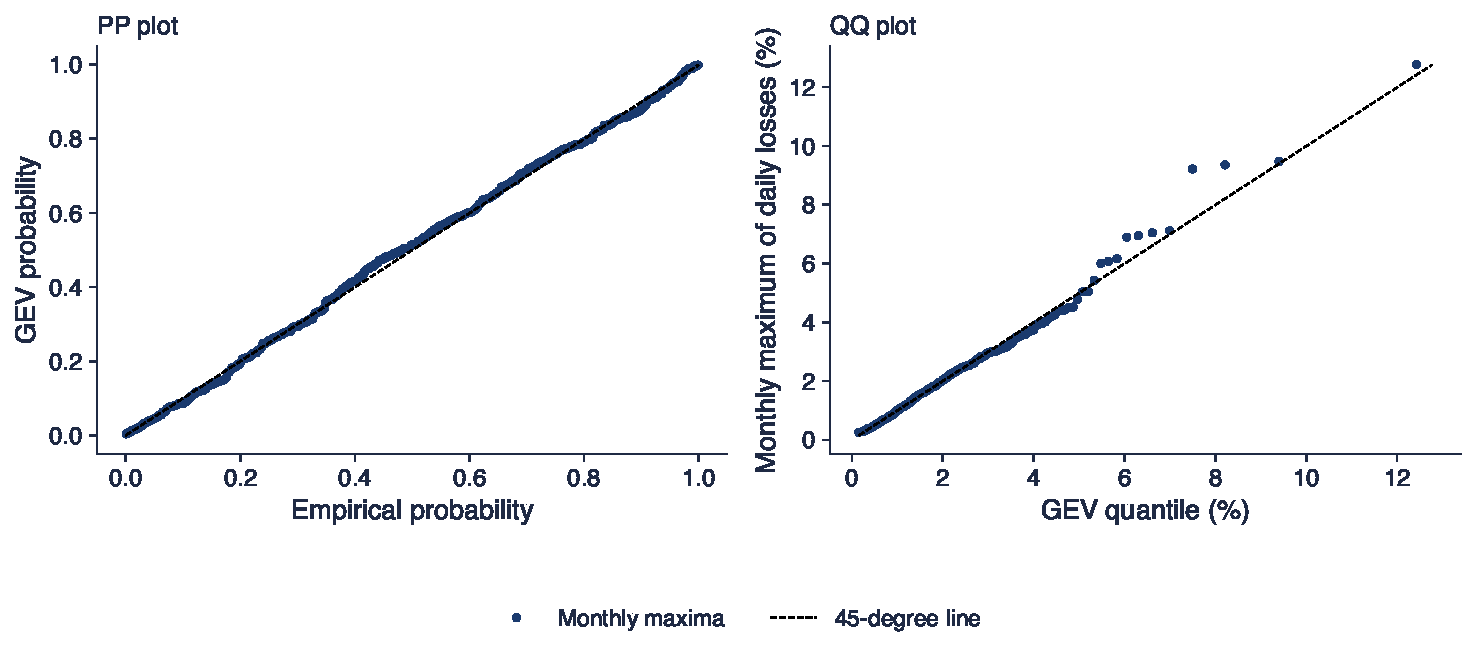
\includegraphics[width=0.97\textwidth,height=0.54\textheight,keepaspectratio]{sfm_ch5_gev_ppqq.pdf}
\end{center}
\vspace{-0.25cm}
\begin{itemize}
    \item \textbf{Graficul PP}: probabilitatea ajustată $H(m_{(i)})$ față de cea empirică $(i - 0{,}5)/n$; \textbf{graficul QQ}: maximele observate față de cuantilele ajustate; S\&P 500
    \item Ambele grafice sînt aproape de prima bisectoare; în graficul QQ, cele cîteva luni extreme (2008, 2020) sînt puțin deasupra: este partea cea mai greu de ajustat
\end{itemize}
\quantlet{SFM\_ch5\_gev\_block\_maxima}{\qlurl{SFM_ch5_gev_block_maxima}}
\end{frame}

\begin{frame}{Return levels (niveluri de revenire)}
\itemsize{\small}
\begin{itemize}
    \item \textbf{Return level} pentru o perioadă de revenire de $T$ ani: nivelul pe care maximul lunar îl depășește, în medie, o dată la $T$ ani
    \begin{itemize}
        \item $z_T = H^{-1}(1 - 1/m)$ cu $m = 12T$ luni: $z_T = \mu + \dfrac{\sigma}{\xi}\big[(-\ln(1 - 1/m))^{-\xi} - 1\big]$
    \end{itemize}
    \item \textbf{Exemplu lucrat}, S\&P 500, $T = 10$ ani: $\hat\xi = 0{,}211$, $\hat\mu = 1{,}311$, $\hat\sigma = 0{,}737$
    \begin{itemize}
        \item $m = 120$; $-\ln(1 - 1/120) = 0{,}00837$; ridicat la $-\hat\xi$: $2{,}747$
        \item $z_{10} = 1{,}311 + (0{,}737/0{,}211)(2{,}747 - 1) = 7{,}4\%$
    \end{itemize}
    \item O pierdere zilnică de circa $7{,}4\%$ în S\&P 500 este un „eveniment de 10 ani”; a fost depășită în 4 luni din 36{,}7 ani
\end{itemize}
\end{frame}

\begin{frame}{Graficul return levels}
\itemsize{\footnotesize}
\begin{center}
    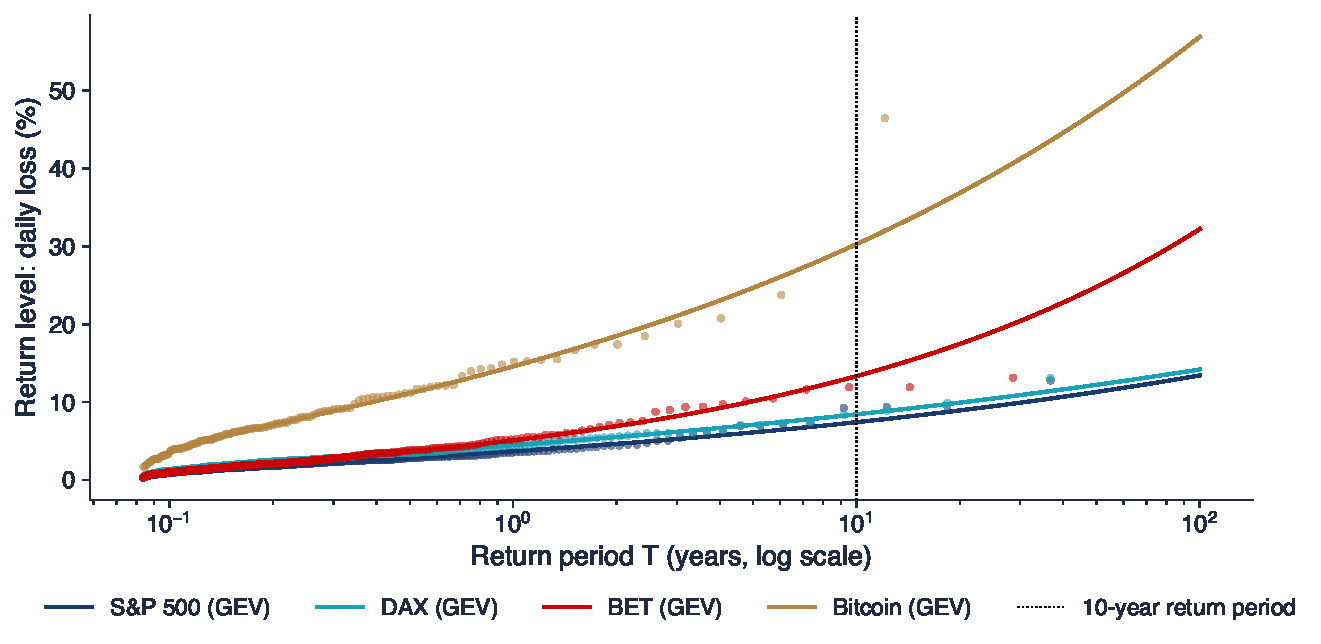
\includegraphics[width=0.97\textwidth,height=0.58\textheight,keepaspectratio]{sfm_ch5_return_levels.pdf}
\end{center}
\vspace{-0.25cm}
\begin{itemize}
    \item Linii: return levels GEV; puncte: maximele lunare observate, la perioadele lor empirice de revenire
    \item Dincolo de lungimea eșantionului (36{,}7 ani pentru S\&P 500, 12 pentru Bitcoin), curbele sînt extrapolare
\end{itemize}
\quantlet{SFM\_ch5\_gev\_block\_maxima}{\qlurl{SFM_ch5_gev_block_maxima}}
\end{frame}

\begin{frame}{Cît de mare este o pierdere de 10 ani?}
\itemsize{\footnotesize}
\begin{center}
\footnotesize
\begin{tabular}{lrrrrrr}
\toprule
& 1 an & 10 ani & interval 95\% & 50 de ani & cea mai mare observată & ani de date \\
\midrule
S\&P 500 & $3{,}7$ & $7{,}4$ & $[6{,}2; 8{,}9]$ & $11{,}3$ & $12{,}8$ & $36{,}7$ \\
DAX & $4{,}5$ & $8{,}4$ & $[7{,}1; 9{,}9]$ & $12{,}2$ & $13{,}1$ & $36{,}7$ \\
BET & $5{,}1$ & $13{,}3$ & $[10{,}3; 17{,}5]$ & $24{,}8$ & $13{,}1$ & $28{,}5$ \\
Bitcoin & $14{,}6$ & $30{,}3$ & $[21{,}2; 41{,}1]$ & $47{,}4$ & $46{,}5$ & $12$ \\
\bottomrule
\end{tabular}
\end{center}
\begin{itemize}
    \item Pierderea zilnică (\%) depășită în medie o dată la $T$ ani; intervalul: bootstrap al maximelor lunare (200 de eșantioane)
    \item BET: cu $\hat\xi = 0{,}36$, nivelul de 50 de ani este $24{,}8\%$, aproape dublul celei mai mari pierderi observate: o mică modificare a lui $\hat\xi$ schimbă mult extremul
    \item Metoda block maxima folosește o singură pierdere pe lună; metoda peaks over threshold folosește toate pierderile mari
\end{itemize}\quantlet{SFM\_ch5\_gev\_block\_maxima}{\qlurl{SFM_ch5_gev_block_maxima}}
\end{frame}

\begin{frame}{Recapitulare: block maxima}
\itemsize{\small}
\begin{itemize}
    \item Maximele variabilelor i.i.d.\ pot converge doar către o lege GEV (Fisher--Tippett--Gnedenko)
    \item $\xi > 0$ Fréchet (groasă, $\alpha = 1/\xi$), $\xi = 0$ Gumbel, $\xi < 0$ Weibull
    \item Maximele lunare ale pierderilor zilnice: Fréchet, $\hat\xi$ între $0{,}17$ și $0{,}36$
    \item Return level: pierderea depășită o dată la $T$ ani; mult dincolo de lungimea eșantionului, este o extrapolare
\end{itemize}
\end{frame}


%=============================================================================
\section{Peaks over threshold și distribuția GPD}
%=============================================================================

\begin{frame}{Peaks over threshold (vîrfuri peste prag)}
\itemsize{\small}
\begin{columns}[T]
\begin{column}{0.58\textwidth}
\begin{itemize}
    \item \textbf{POT} (peaks over threshold, vîrfuri peste prag): fixăm un prag înalt $u$ și păstrăm fiecare pierdere de peste el
    \begin{itemize}
        \item \textbf{excesul} peste $u$: $Y = L - u$, știind că $L > u$
        \item distribuția excesului: $F_u(y) = P(L - u \le y \mid L > u)$
    \end{itemize}
    \item Folosește toate pierderile mari, nu una pe bloc: mai multe date în coadă
    \item Metoda care stă la baza majorității estimărilor EVT pentru VaR și ES \refMF, \refQRM
\end{itemize}
\end{column}
\begin{column}{0.38\textwidth}
\centering

\includegraphics[height=0.36\textheight]{ch5_dehaan_1987.jpg}\\[1mm]
\imgcap{Laurens de Haan, Oberwolfach, 1987}
\imgcredit{https://commons.wikimedia.org/wiki/File:Laurens_de_haan.jpg}{Foto: Konrad Jacobs (1987), Oberwolfach Photo Collection; CC BY-SA 2.0 de; Wikimedia Commons}
\end{column}
\end{columns}
\end{frame}

\begin{frame}{Teorema Pickands--Balkema--de Haan}
\itemsize{\small}
\begin{itemize}
    \item Dacă maximele lui $L$ converg către o GEV cu forma $\xi$, atunci pentru praguri înalte
    \begin{itemize}
        \item $F_u(y) \approx G_{\xi, \beta(u)}(y)$, \textbf{GPD} (generalised Pareto distribution, distribuția Pareto generalizată) \refPickands, \refBdH
    \end{itemize}
    \item $G_{\xi, \beta}(y) = 1 - \Big(1 + \xi\,\dfrac{y}{\beta}\Big)^{-1/\xi}$, $y \ge 0$ (pentru $\xi < 0$: $y \le -\beta/\xi$); $\xi = 0$: $1 - e^{-y/\beta}$
    \begin{itemize}
        \item forma $\xi$: \textbf{aceeași} ca la GEV; scala $\beta > 0$ depinde de $u$
        \item $\xi > 0$: coadă de tip Pareto cu $\alpha = 1/\xi$; $\xi = 0$: exponențială; $\xi < 0$: mărginită
    \end{itemize}
    \item Momentele GPD: media $\beta/(1 - \xi)$ dacă $\xi < 1$; varianța finită dacă $\xi < 1/2$
    \begin{itemize}
        \item funcția mean excess a unei GPD: $e(v) = \dfrac{\beta + \xi(v - u)}{1 - \xi}$, o dreaptă în $v > u$, ca în Secțiunea 4
    \end{itemize}
\end{itemize}
\end{frame}

\begin{frame}{Densități și cozi GPD}
\itemsize{\footnotesize}
\begin{center}
    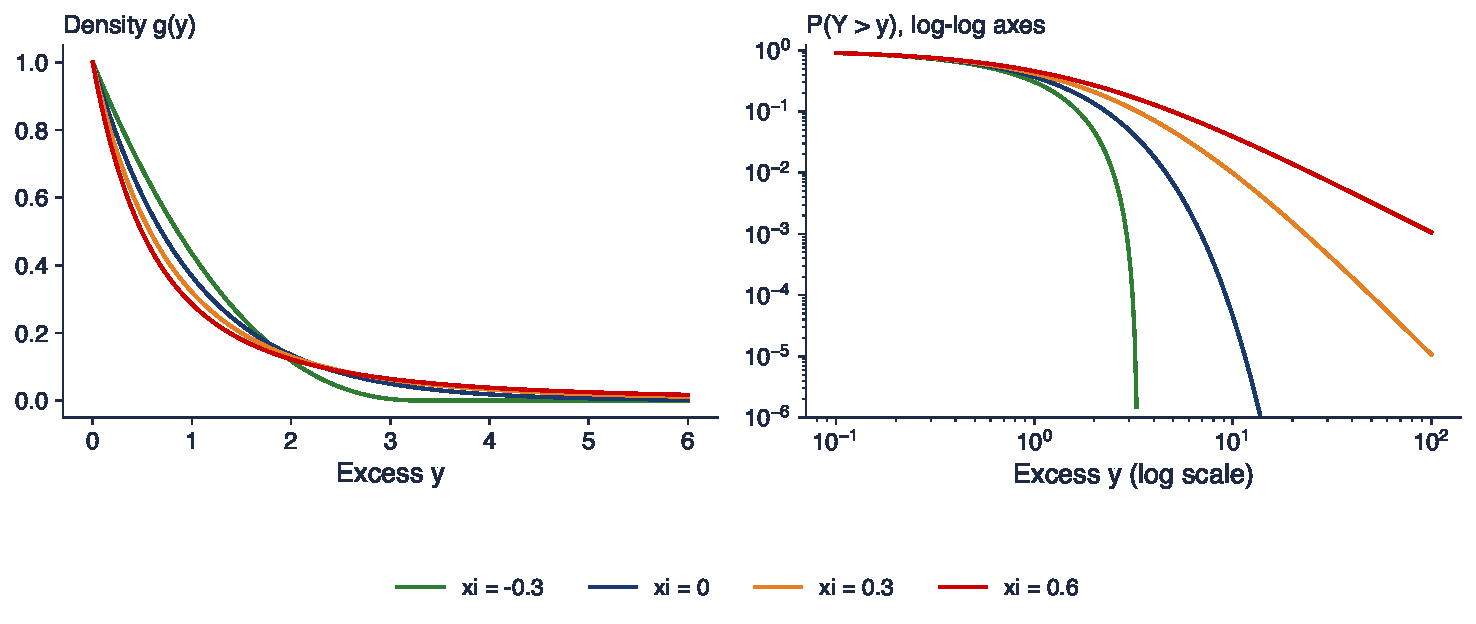
\includegraphics[width=0.97\textwidth,height=0.56\textheight,keepaspectratio]{sfm_ch5_gpd_densities.pdf}
\end{center}
\vspace{-0.25cm}
\begin{itemize}
    \item $\beta = 1$; densitățile seamănă lîngă 0, cozile nu: pe axe log-log, doar $\xi > 0$ dă drepte
    \item $\xi = 0{,}3$ corespunde unui indice de coadă $\alpha \approx 3{,}3$, apropiat de cel al randamentelor acțiunilor
\end{itemize}
\quantlet{SFM\_ch5\_pot\_gpd}{\qlurl{SFM_ch5_pot_gpd}}
\end{frame}

\begin{frame}{Alegerea pragului}
\itemsize{\small}
\begin{itemize}
    \item Același compromis ca la alegerea lui $k$ pentru estimatorul Hill
    \begin{itemize}
        \item $u$ prea jos: aproximarea GPD este slabă (deplasare); $u$ prea sus: puține excese (varianță)
    \end{itemize}
    \item Instrumente grafice
    \begin{itemize}
        \item graficul mean excess: aproximativ liniar peste $u$
        \item graficul stabilității parametrilor: $\hat\xi$ nu ar trebui să se schimbe mult cînd $u$ crește în continuare
    \end{itemize}
    \item Regula folosită aici: $u =$ cuantila de 90\% a pierderilor, adică cele mai mari 10\% dintre pierderi
    \begin{itemize}
        \item \refMF\ folosesc $k = 100$ de excese în ferestre de $n = 1000$ de zile, aceeași proporție
        \item pentru S\&P 500: $u = 1{,}16\%$ și $N_u = 924$ excese
    \end{itemize}
\end{itemize}
\end{frame}

\begin{frame}{Stabilitatea parametrilor}
\itemsize{\footnotesize}
\begin{center}
    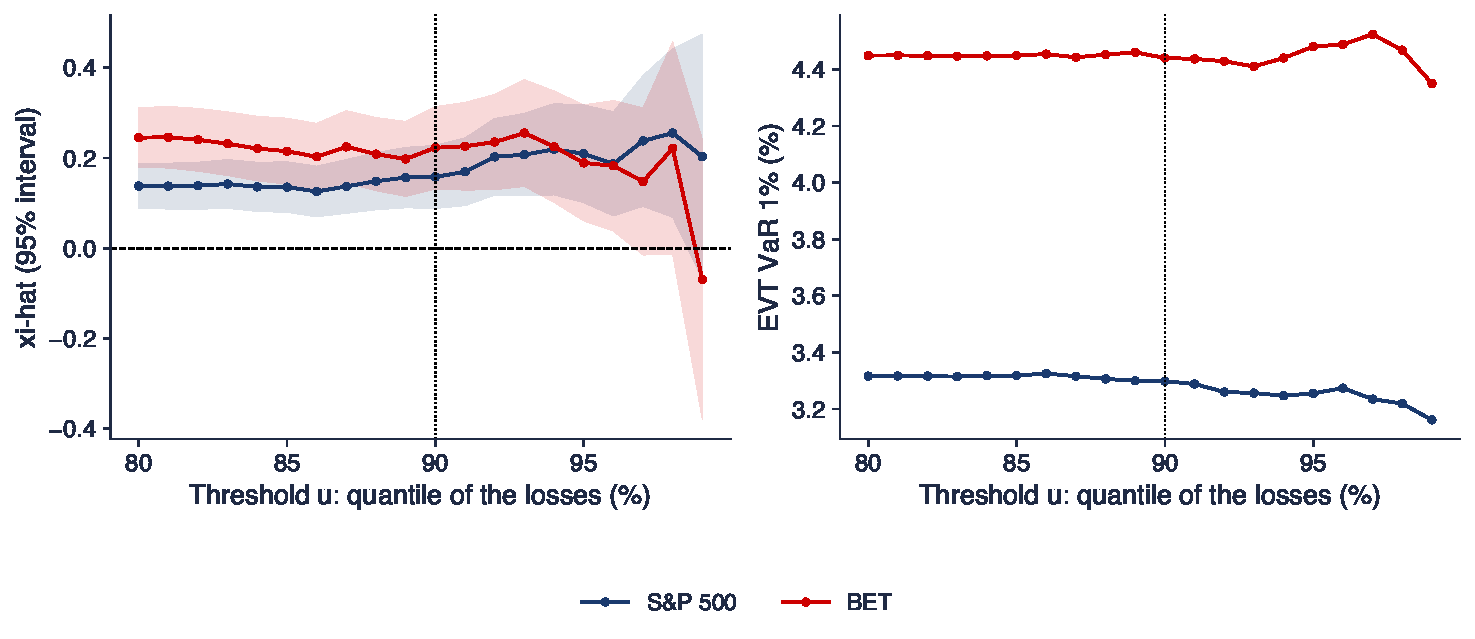
\includegraphics[width=0.97\textwidth,height=0.54\textheight,keepaspectratio]{sfm_ch5_threshold_stability.pdf}
\end{center}
\vspace{-0.25cm}
\begin{itemize}
    \item Stînga: $\hat\xi$ cu interval de 95\% pentru $u$ de la cuantila de 80\% la cea de 99\%; dreapta: VaR 1\% EVT pentru aceleași praguri
    \item Între cuantilele de 85\% și 95\%: S\&P 500 $\hat\xi \in [0{,}13; 0{,}22]$, VaR 1\% $\in [3{,}25; 3{,}33]\%$; VaR se modifică foarte puțin
\end{itemize}
\quantlet{SFM\_ch5\_pot\_gpd}{\qlurl{SFM_ch5_pot_gpd}}
\end{frame}

\begin{frame}{Ajustări GPD peste cuantila de 90\%}
\itemsize{\footnotesize}
\begin{center}
\footnotesize
\begin{tabular}{lrrrrrrr}
\toprule
& $n$ & $u$ (\%) & $N_u$ & $\hat\xi$ & SE & $\hat\beta$ & $1/\hat\xi$ \\
\midrule
S\&P 500 & 9\,240 & $1{,}16$ & 924 & $0{,}16$ & $0{,}04$ & $0{,}769$ & $6{,}3$ \\
DAX & 9\,288 & $1{,}50$ & 929 & $0{,}12$ & $0{,}04$ & $0{,}927$ & $8{,}5$ \\
BET & 7\,243 & $1{,}38$ & 725 & $0{,}22$ & $0{,}05$ & $1{,}018$ & $4{,}5$ \\
Bitcoin & 4\,384 & $3{,}33$ & 439 & $0{,}12$ & $0{,}05$ & $2{,}663$ & $8{,}5$ \\
\bottomrule
\end{tabular}
\end{center}
\begin{itemize}
    \item Verosimilitate maximă pe excesele $L - u$ \refDS; SE din curbura log-verosimilității
    \item $\hat\xi$ între $0{,}12$ și $0{,}22$: cozi groase cu varianță finită ($\xi < 0{,}5$) pentru toate cele patru serii
    \item $1/\hat\xi$ este mai mare decît $\hat\alpha$ Hill (2,5\% din pierderi): peste cuantila de 90\%, o GPD cu scala liberă $\beta$ are nevoie de un $\xi$ mai mic; indicele de coadă este greu de estimat precis, deci raportați mai mulți estimatori
\end{itemize}\quantlet{SFM\_ch5\_pot\_gpd}{\qlurl{SFM_ch5_pot_gpd}}
\end{frame}

\begin{frame}{Se potrivește GPD? Grafice PP și QQ}
\itemsize{\footnotesize}
\begin{center}
    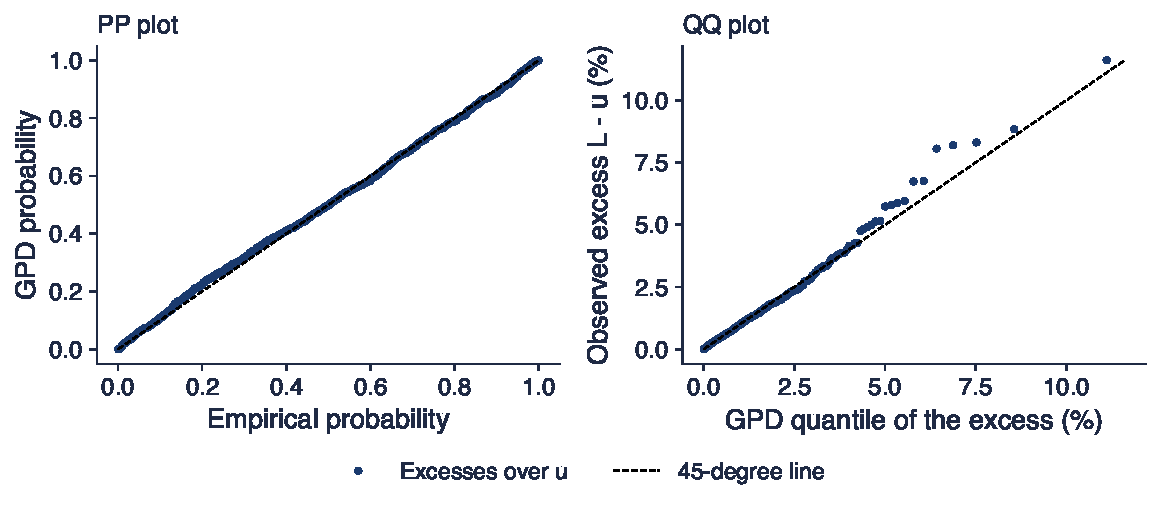
\includegraphics[width=0.97\textwidth,height=0.54\textheight,keepaspectratio]{sfm_ch5_gpd_ppqq.pdf}
\end{center}
\vspace{-0.25cm}
\begin{itemize}
    \item Excesele S\&P 500 peste $u$: punctele graficului PP stau pe dreaptă; cele ale graficului QQ, pînă la excese de circa 4\%
    \item Cel mai mare exces ($11{,}6\%$, martie 2020) față de o cuantilă ajustată de $11{,}1\%$; portat din Quantlet-urile SFE SFEtailGPareto\_pp și \_qq
\end{itemize}
\quantlet{SFM\_ch5\_pot\_gpd}{\qlurl{SFM_ch5_pot_gpd}}
\end{frame}

\begin{frame}{De la GPD la coada pierderilor}
\itemsize{\small}
\begin{itemize}
    \item Pentru $x > u$: $P(L > x) = P(L > u)\,P(L > x \mid L > u)$
    \begin{itemize}
        \item estimăm $P(L > u)$ prin $N_u/n$ și $P(L > x \mid L > u)$ prin GPD
    \end{itemize}
    \item \textbf{Estimatorul cozii}: $\hat{\bar F}(x) = \dfrac{N_u}{n}\Big(1 + \hat\xi\,\dfrac{x - u}{\hat\beta}\Big)^{-1/\hat\xi}$, $x > u$
    \item În interiorul eșantionului folosim datele istorice; dincolo de el, o lege putere ajustată
    \begin{itemize}
        \item modelul se folosește doar acolo unde este justificat: peste $u$
    \end{itemize}
    \item Inversarea lui $\hat{\bar F}(x) = p$ dă VaR; integrarea dincolo de el dă ES (Secțiunea 7)
\end{itemize}
\end{frame}

\begin{frame}{Cozile ajustate}
\itemsize{\footnotesize}
\begin{center}
    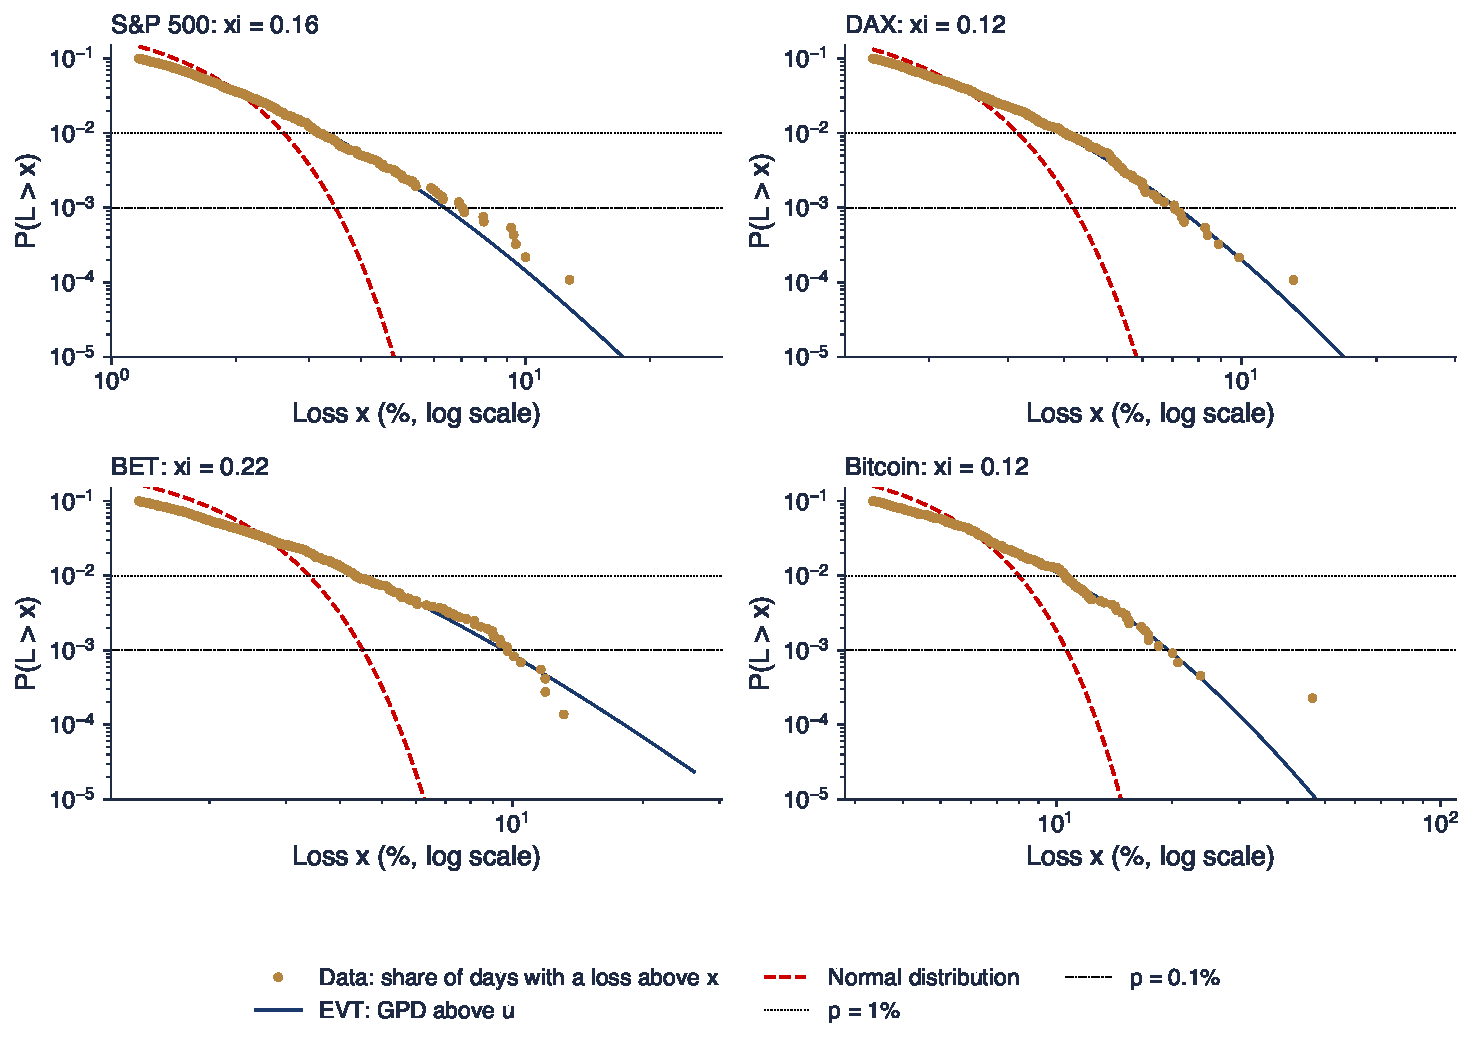
\includegraphics[width=0.97\textwidth,height=0.66\textheight,keepaspectratio]{sfm_ch5_tail_fit.pdf}
\end{center}
\vspace{-0.25cm}
\begin{itemize}
    \item Puncte: proporția zilelor cu o pierdere peste $x$ (peste $u$); albastru: estimatorul EVT al cozii; roșu: distribuția Normală; linii punctate la $p = 1\%$ și $0{,}1\%$
    \item GPD urmează datele pînă la $10^{-4}$; coada distribuției Normale se îndepărtează de ele înainte de $p = 1\%$
\end{itemize}
\quantlet{SFM\_ch5\_pot\_gpd}{\qlurl{SFM_ch5_pot_gpd}}
\end{frame}

\begin{frame}{Înapoi la crahuri: cît de des?}
\itemsize{\footnotesize}
\begin{center}
\footnotesize
\begin{tabular}{llrrr}
\toprule
& ziua & pierdere (\%) & distribuția Normală: o dată la (ani) & EVT: o dată la (ani) \\
\midrule
S\&P 500 & 16 martie 2020 & ${-12{,}8}$ & $10^{27}$ & $89$ \\
DAX & 12 martie 2020 & ${-13{,}1}$ & $10^{19}$ & $85$ \\
BET & 7 ianuarie 2009 & ${-13{,}1}$ & $10^{16}$ & $12$ \\
Bitcoin & 12 martie 2020 & ${-46{,}5}$ & $10^{38}$ & $237$ \\
S\&P 500, Lunea Neagră & 19 octombrie 1987 & $-22{,}3$ & $10^{84}$ & $1\,600$ \\
\bottomrule
\end{tabular}
\end{center}
\begin{itemize}
    \item Timpul de așteptare EVT: $1/(\hat{\bar F}(x) \times 252)$ ani (365 pentru Bitcoin), cu ajustarea POT pe întregul eșantion
    \item Pentru EVT, zilele COVID-19 sînt evenimente rare, dar plauzibile, de tipul „o dată într-o viață”; pentru distribuția Normală sînt imposibile
    \item 1987 este în afara datelor noastre: EVT îl extrapolează la un timp de așteptare de circa 1\,600 de ani, cu o incertitudine mare
\end{itemize}\quantlet{SFM\_ch5\_pot\_gpd}{\qlurl{SFM_ch5_pot_gpd}}
\end{frame}

\begin{frame}{Recapitulare: peaks over threshold}
\itemsize{\small}
\begin{itemize}
    \item Excesele peste un prag înalt urmează aproximativ o GPD (Pickands--Balkema--de Haan)
    \item Aceeași formă $\xi$ ca la GEV; $\xi > 0$: coadă de tip putere cu $\alpha = 1/\xi$
    \item Pragul: mean excess și stabilitatea parametrilor; aici cuantila de 90\%
    \item Estimatorul cozii: datele pînă la $u$, GPD dincolo de $u$; verificare cu grafice PP și QQ
\end{itemize}
\end{frame}


%=============================================================================
\section{VaR și ES prin teoria valorilor extreme}
%=============================================================================

\begin{frame}{VaR și ES: definiții}
\itemsize{\small}
\begin{itemize}
    \item Pierderile $L = -r$ cu funcția de repartiție $F_L$; nivelul $p$ (de ex.\ $p = 1\%$)
    \begin{itemize}
        \item $\mathrm{VaR}_p = F_L^{-1}(1 - p) = -q_p(r)$: pierderea depășită cu probabilitatea $p$
        \item $\mathrm{ES}_p = \dfrac{1}{p}\displaystyle\int_0^p \mathrm{VaR}_s\,ds = E[L \mid L \ge \mathrm{VaR}_p]$ pentru distribuții continue
    \end{itemize}
    \item Trei moduri de a le estima din pierderile zilnice
    \begin{itemize}
        \item \textbf{simularea istorică}: cuantila empirică și media pierderilor de dincolo de ea
        \item \textbf{distribuția Normală}: $\mathrm{VaR}_p = \hat\mu_L + \hat\sigma z_{1-p}$, $\mathrm{ES}_p = \hat\mu_L + \hat\sigma\,\varphi(z_{1-p})/p$ ($\varphi$: densitatea distribuției Normale standard)
        \item \textbf{EVT (POT)}: inversăm estimatorul cozii
    \end{itemize}
    \item Nivelurile folosite în practică: VaR 1\% (zilnic, backtesting Basel), ES 2,5\% \refBasel, VaR 0,1\% (stres)
\end{itemize}
\end{frame}

\begin{frame}{Formulele EVT pentru VaR și ES}
\itemsize{\small}
\begin{itemize}
    \item Rezolvăm $\dfrac{N_u}{n}\Big(1 + \xi\,\dfrac{x - u}{\beta}\Big)^{-1/\xi} = p$ în raport cu $x$
    \begin{itemize}
        \item $\mathrm{VaR}_p = u + \dfrac{\beta}{\xi}\Big[\Big(\dfrac{n p}{N_u}\Big)^{-\xi} - 1\Big]$, valabil pentru $p < N_u/n$
    \end{itemize}
    \item Excesul peste $\mathrm{VaR}_p$ are tot distribuție GPD, cu același $\xi$: media lui este $(\beta + \xi(\mathrm{VaR}_p - u))/(1 - \xi)$
    \begin{itemize}
        \item $\mathrm{ES}_p = \dfrac{\mathrm{VaR}_p}{1 - \xi} + \dfrac{\beta - \xi u}{1 - \xi}$, valabil pentru $\xi < 1$ \refMF
    \end{itemize}
    \item Cu $\xi > 0$, ES este un multiplu fix al VaR în coada îndepărtată: $\mathrm{ES}_p/\mathrm{VaR}_p \to 1/(1 - \xi)$
    \item Portat din Quantlet-ul SFE var\_pot (estimări VaR cu modelul POT)
\end{itemize}
\end{frame}

\begin{frame}{Exemplu lucrat: S\&P 500, pas cu pas}
\itemsize{\small}
\begin{itemize}
    \item Ajustarea: $n = 9\,240$, $u = 1{,}163\%$, $N_u = 924$ ($10{,}0\%$), $\hat\xi = 0{,}158$, $\hat\beta = 0{,}769$, $\hat\beta/\hat\xi = 4{,}860$
    \item \textbf{VaR 1\%}: $np/N_u = 0{,}100$; $0{,}100^{-\hat\xi} = 1{,}439$
    \begin{itemize}
        \item $\mathrm{VaR}_{1\%} = 1{,}163 + 4{,}860\,(1{,}439 - 1) = 3{,}30\%$
    \end{itemize}
    \item \textbf{ES 2,5\%}: $np/N_u = 0{,}250$, $\mathrm{VaR}_{2,5\%} = 1{,}163 + 4{,}860\,(1{,}245 - 1) = 2{,}35\%$
    \begin{itemize}
        \item $\mathrm{ES}_{2,5\%} = \dfrac{2{,}35 + 0{,}769 - 0{,}158 \times 1{,}163}{1 - 0{,}158} = 3{,}49\%$
    \end{itemize}
    \item \textbf{VaR 0,1\%}: $np/N_u = 0{,}010$, $0{,}010^{-\hat\xi} = 2{,}072$, $\mathrm{VaR}_{0,1\%} = 6{,}37\%$
\end{itemize}
\end{frame}

\begin{frame}{VaR 1\% și ES 2,5\%: trei metode}
\itemsize{\footnotesize}
\begin{center}
\footnotesize
\begin{tabular}{l|rrr|rrr}
\toprule
& \multicolumn{3}{c|}{VaR 1\% (\%)} & \multicolumn{3}{c}{ES 2,5\% (\%)} \\ & EVT & istoric & Normal & EVT & istoric & Normal \\
\midrule
S\&P 500 & $3{,}30$ & $3{,}15$ & $2{,}60$ & $3{,}49$ & $3{,}48$ & $2{,}62$ \\
DAX & $3{,}95$ & $4{,}02$ & $3{,}16$ & $4{,}13$ & $4{,}15$ & $3{,}18$ \\
BET & $4{,}44$ & $4{,}33$ & $3{,}39$ & $4{,}81$ & $4{,}80$ & $3{,}41$ \\
Bitcoin & $10{,}38$ & $10{,}51$ & $7{,}99$ & $10{,}90$ & $10{,}84$ & $8{,}03$ \\
\bottomrule
\end{tabular}
\end{center}
\begin{itemize}
    \item La aceste niveluri, EVT și simularea istorică diferă cu cel mult $0{,}14$ puncte procentuale: există destule date la 1\% și 2,5\%
    \item Distribuția Normală subestimează riscul: VaR 1\% EVT este cu $27\%$ mai mare pentru S\&P 500 și cu $31\%$ mai mare pentru BET; ES 2,5\% cu o marjă asemănătoare
\end{itemize}\quantlet{SFM\_ch5\_evt\_var}{\qlurl{SFM_ch5_evt_var}}
\end{frame}

\begin{frame}{Departe în coadă: VaR 0,1\%}
\itemsize{\footnotesize}
\begin{center}
\scriptsize
\begin{tabular}{lrrrrr}
\toprule
& EVT (POT) & Hill & istoric & Normal & cea mai mare pierdere \\
\midrule
S\&P 500 & $6{,}37$ & $6{,}92$ & $6{,}94$ & $3{,}47$ & $12{,}8$ \\
DAX & $7{,}17$ & $8{,}37$ & $6{,}97$ & $4{,}21$ & $13{,}1$ \\
BET & $9{,}56$ & $10{,}69$ & $9{,}64$ & $4{,}52$ & $13{,}1$ \\
Bitcoin & $19{,}61$ & $23{,}30$ & $18{,}05$ & $10{,}65$ & $46{,}5$ \\
OMV Petrom (SNP) & $8{,}89$ & $9{,}29$ & $8{,}32$ & $4{,}94$ & $15{,}8$ \\
BRD & $8{,}39$ & $8{,}93$ & $7{,}85$ & $5{,}07$ & $18{,}2$ \\
Banca Transilvania (TLV) & $10{,}68$ & $12{,}10$ & $10{,}50$ & $5{,}35$ & $22{,}2$ \\
Transgaz (TGN) & $8{,}29$ & $9{,}18$ & $8{,}23$ & $4{,}68$ & $10{,}1$ \\
\bottomrule
\end{tabular}
\end{center}
\begin{itemize}
    \item VaR 0,1\% (\%): pierderea depășită într-o zi din 1\,000; acțiunile BVB din 2010
    \item VaR EVT este de circa $1{,}8$ ori mai mare decît cel Normal pentru S\&P 500 și de $2{,}1$ ori pentru BET
    \item VaR 0,1\% istoric se bazează doar pe cele mai mari 3--9 pierderi; EVT și Hill le netezesc cu un model al cozii
\end{itemize}\quantlet{SFM\_ch5\_evt\_var}{\qlurl{SFM_ch5_evt_var}}
\end{frame}

\begin{frame}{În afara eșantionului: estimare pînă în 2019, test 2020--2026}
\itemsize{\footnotesize}
\begin{center}
    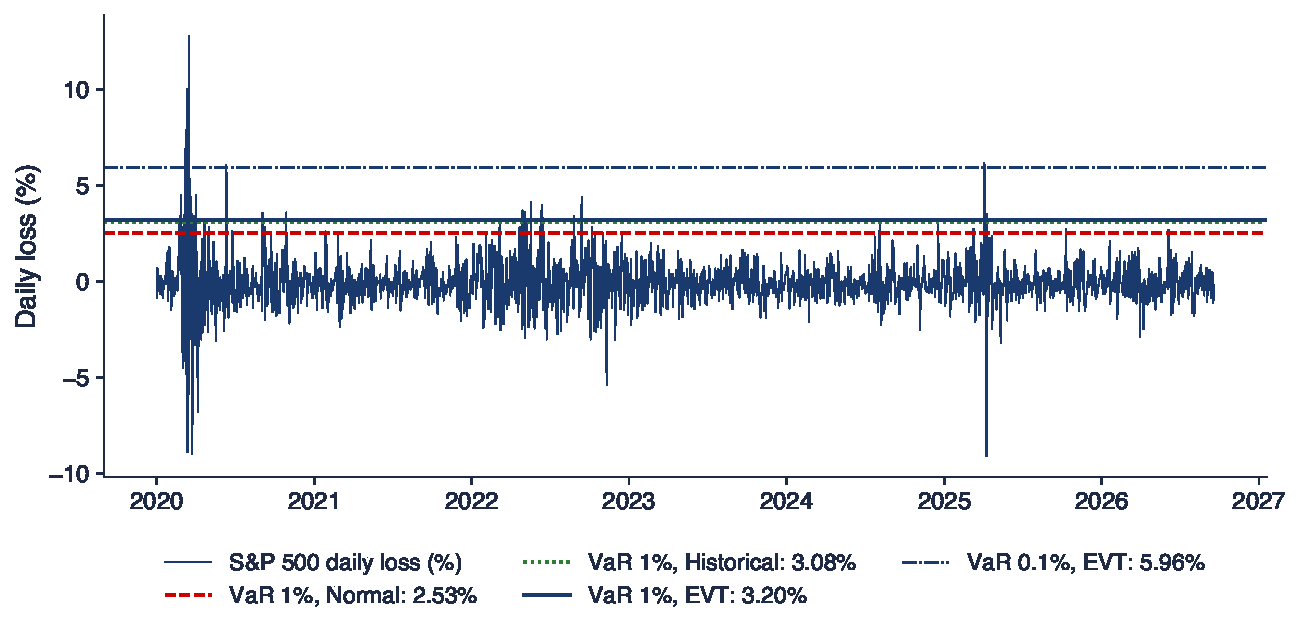
\includegraphics[width=0.97\textwidth,height=0.58\textheight,keepaspectratio]{sfm_ch5_oos.pdf}
\end{center}
\vspace{-0.25cm}
\begin{itemize}
    \item Pierderile zilnice ale S\&P 500 după 2019, comparate cu VaR 1\% al celor trei metode, toate estimate pe perioada 1990--2019
    \item Un VaR 1\% bun este depășit în circa 1\% din zilele de test, aici $16{,}9$ zile
\end{itemize}
\quantlet{SFM\_ch5\_evt\_var}{\qlurl{SFM_ch5_evt_var}}
\end{frame}

\begin{frame}{Numărarea depășirilor}
\itemsize{\footnotesize}
\begin{center}
\scriptsize
\begin{tabular}{lr|rrrr|rrrr}
\toprule
& & \multicolumn{4}{c|}{VaR 1\%} & \multicolumn{4}{c}{VaR 0,1\%} \\ & zile de test & așteptat & EVT & ist. & Normal & așteptat & EVT & ist. & Normal \\
\midrule
S\&P 500 & 1\,687 & $16{,}9$ & 25 & 26 & 44 & $1{,}7$ & 5 & 3 & 23 \\
DAX & 1\,710 & $17{,}1$ & 15 & 12 & 31 & $1{,}7$ & 2 & 2 & 8 \\
BET & 1\,674 & $16{,}7$ & 4 & 5 & 13 & $1{,}7$ & 0 & 1 & 4 \\
Bitcoin & 2\,453 & $24{,}5$ & 8 & 10 & 23 & $2{,}5$ & 1 & 1 & 8 \\
\bottomrule
\end{tabular}
\end{center}
\begin{itemize}
    \item VaR Normal este depășit mult prea des, mai ales la 0,1\%: 23 de zile în loc de $1{,}7$ pentru S\&P 500
    \item VaR EVT și VaR istoric sînt apropiate între ele; S\&P 500 peste valoarea așteptată (episodul din 2020), BET sub ea (ani liniștiți)
    \item Un VaR estimat o singură dată ignoră variația volatilității în timp: EVT condiționată (GARCH + POT) \refMF, Capitolele 9 și 10
\end{itemize}\quantlet{SFM\_ch5\_evt\_var}{\qlurl{SFM_ch5_evt_var}}
\end{frame}

\begin{frame}{Posibilitățile și limitele EVT}
\itemsize{\small}
\begin{itemize}
    \item \textbf{Poate}: să ofere un model teoretic fundamentat al cozii și să extrapoleze dincolo de cea mai mare pierdere observată
    \begin{itemize}
        \item VaR și ES stabile la 0,1\%, acolo unde simularea istorică are doar cîteva puncte
    \end{itemize}
    \item \textbf{Nu poate}: să elimine incertitudinea cozii îndepărtate
    \begin{itemize}
        \item $\hat\xi$ are aici o eroare standard de $0{,}04$--$0{,}06$; return levels dincolo de eșantion au intervale largi
    \end{itemize}
    \item \textbf{Presupune}: pierderi i.i.d., sau măcar o coadă stabilă în timp
    \begin{itemize}
        \item aplicați EVT pe randamente împărțite la o volatilitate GARCH (Capitolul 9) pentru riscul zilnic; pentru o alternativă, vedeți ES calculat pe baza entropiei \refPeleA
    \end{itemize}
    \item Sinteze despre EVT în finanțe: \refRocco; \refQRM, cap.~5
\end{itemize}
\end{frame}

\begin{frame}{Recapitulare: VaR și ES prin EVT}
\itemsize{\small}
\begin{itemize}
    \item $\mathrm{VaR}_p = u + \frac{\beta}{\xi}[(np/N_u)^{-\xi} - 1]$; $\mathrm{ES}_p = (\mathrm{VaR}_p + \beta - \xi u)/(1 - \xi)$
    \item VaR 1\% și ES 2,5\%: EVT $\approx$ simularea istorică; distribuția Normală subestimează
    \item VaR 0,1\%: VaR EVT este de circa două ori VaR-ul Normal; simularea istorică se bazează pe cîteva zile
    \item În afara eșantionului: VaR Normal eșuează; EVT necondiționată ignoră regimurile de volatilitate
\end{itemize}
\end{frame}


%=============================================================================
\section{AI pentru descoperire științifică}
%=============================================================================

\begin{frame}{O întrebare deschisă}
\itemsize{\small}
\begin{itemize}
    \item \textbf{S-a schimbat coada pierderilor BET pe măsură ce piața din București a crescut?}
    \begin{itemize}
        \item indicele Hill, $k = 2{,}5\%$ din $n$: 1997--2009: $\hat\alpha = 2{,}90$ (SE pe blocuri $0{,}33$); 2010--2026: $\hat\alpha = 2{,}16$ ($0{,}27$)
        \item $z = -1{,}73$: o coadă mai groasă după 2010, dar nesemnificativă la 5\%
    \end{itemize}
    \item De ce rămîne deschisă: pragul a scăzut de la $3{,}95\%$ la $2{,}01\%$ odată cu volatilitatea; schimbarea este în coadă sau în volatilitate?
    \item Instrumentele AI pot accelera un astfel de studiu; nu înlocuiesc verificarea lui \refWang
\end{itemize}\quantlet{SFM\_ch5\_hill}{\qlurl{SFM_ch5_hill}}
\end{frame}

\begin{frame}{Contribuția posibilă a AI}
\itemsize{\small}
\begin{itemize}
    \item \textbf{Literatura}: lista studiilor despre indicii de coadă pe piețele emergente și rezumatul metodelor lor
    \item \textbf{Cod}: o primă versiune a unei analize Hill și POT pe ferestre mobile, cu intervale bootstrap pe blocuri
    \item \textbf{Robustețe}: alte praguri, randamente standardizate cu GARCH, alți indici BVB
    \item Exemplu de prompt
    \begin{itemize}
        \item \aiprompt{Write a Python function that computes the Hill tail index of daily BET losses with k = 2.5\% of n on rolling 5-year windows, with moving-block bootstrap standard errors (blocks of 20 days).}
    \end{itemize}
\end{itemize}
\end{frame}

\begin{frame}{Verificări necesare}
\itemsize{\small}
\begin{itemize}
    \item Semnul: pierderile sînt $-r$; o estimare Hill pe randamente, nu pe pierderi, măsoară cîștigurile
    \item Parametrizarea: \texttt{genextreme} din scipy folosește $c = -\xi$; \texttt{genpareto} folosește $c = \xi$
    \item Regula pentru $k$ sau $u$ se fixează înainte de a vedea rezultatul, nu se ajustează pentru a obține o schimbare semnificativă
    \item Ferestrele mobile se suprapun: estimările lor nu sînt teste independente
    \item Referințele: fiecare lucrare citată trebuie să existe; verificați DOI-ul
\end{itemize}
\end{frame}

\begin{frame}{Idee de proiect}
\itemsize{\small}
\begin{itemize}
    \item \textbf{Întrebarea}: este coada pierderilor BET mai subțire sau mai groasă azi decît înainte de 2010, după ce eliminăm volatilitatea?
    \begin{itemize}
        \item date: închiderile zilnice BET din 1997 (EODHD); opțional BET-TR din 2014
    \end{itemize}
    \item Pași
    \begin{itemize}
        \item Hill și POT ($u$ la cuantila de 90\%) pentru cele două perioade, cu intervale bootstrap pe blocuri
        \item repetați pe randamente împărțite la o volatilitate mobilă pe 60 de zile: se menține diferența?
        \item comparați cu S\&P 500 pe aceleași perioade
    \end{itemize}
    \item Rezultat: un tabel, un grafic și un paragraf despre concluziile pe care datele le susțin și pe care nu le susțin
    \item Declarați orice folosire a AI și listați erorile AI pe care le-ați corectat
\end{itemize}
\end{frame}


%=============================================================================
\section{Rezumat}
%=============================================================================

\begin{frame}{Idei principale}
\itemsize{\small}
\begin{itemize}
    \item Pierderile zilnice au cozi de tip putere cu indicele $\alpha \approx 3$: varianță finită, aplatizare infinită
    \item Hill: indicele de coadă din cele mai mari $k$ pierderi; $k$ ales cu ajutorul graficului Hill; SE prin bootstrap pe blocuri
    \item Block maxima $\to$ GEV; excesele peste un prag $\to$ GPD; aceeași formă $\xi = 1/\alpha$
    \item Verificați fiecare ajustare cu mean excess, stabilitatea parametrilor, grafice PP și QQ
    \item VaR și ES EVT: apropiate de cele istorice la 1\% și 2,5\%, mult peste valorile distribuției Normale la 0,1\%
    \item Extrapolarea mult dincolo de date rămîne incertă: raportați intervale
\end{itemize}
\end{frame}

\begin{frame}{Formule de reținut}
\itemsize{\small}
{\renewcommand{\arraystretch}{1.45}\begin{center}
\scriptsize
\begin{tabular}{ll}
\toprule
\textbf{Mărimea} & \textbf{Formula} \\
\midrule
Variație regulată & $P(L > x) = x^{-\alpha}\ell(x)$, \quad $P(L > tx)/P(L > x) \to t^{-\alpha}$ \\
Hill & $\hat\alpha_k = [\frac1k\sum_{i=1}^k \ln(L_{(i)}/L_{(k+1)})]^{-1}$, \quad $\mathrm{SE} \approx \hat\alpha/\sqrt{k}$ \\
Cuantila Hill & $\hat x_p = L_{(k+1)}(k/(np))^{1/\hat\alpha}$ \\
Mean excess & $e(u) = E[L - u \mid L > u]$; \quad GPD: $(\beta + \xi(v - u))/(1 - \xi)$ \\
GEV & $H(x) = \exp\{-[1 + \xi(x - \mu)/\sigma]^{-1/\xi}\}$ \\
Return level & $z_T = \mu + \frac{\sigma}{\xi}[(-\ln(1 - \frac{1}{12T}))^{-\xi} - 1]$ \\
GPD & $G(y) = 1 - (1 + \xi y/\beta)^{-1/\xi}$ \\
VaR (POT) & $u + \frac{\beta}{\xi}[(np/N_u)^{-\xi} - 1]$ \\
ES (POT) & $(\mathrm{VaR}_p + \beta - \xi u)/(1 - \xi)$ \\
\bottomrule
\end{tabular}
\end{center}
}
\end{frame}

\begin{frame}{Verificați-vă}
\itemsize{\small}
\begin{itemize}
    \item \textbf{Întrebare}: o ajustare GPD dă $\hat\xi = 0{,}25$; ce momente ale pierderilor există?
    \begin{itemize}
        \item \textbf{Răspuns}: $\alpha = 1/\xi = 4$: există media, varianța și asimetria; aplatizarea nu (doar $m < 4$)
    \end{itemize}
    \item \textbf{Întrebare}: de ce folosim cele mai mari 2,5\% dintre pierderi și nu toate pierderile pentru estimatorul Hill?
    \begin{itemize}
        \item \textbf{Răspuns}: legea putere este valabilă doar în coadă; dacă includem corpul distribuției, $\hat\alpha$ este deplasat
    \end{itemize}
    \item \textbf{Întrebare}: este VaR 0,1\% prin simulare istorică fiabil cu 10 ani de date?
    \begin{itemize}
        \item \textbf{Răspuns}: nu: circa 2\,500 de zile conțin doar 2--3 pierderi dincolo de el; EVT folosește întreaga coadă
    \end{itemize}
    \item Urmează: \sfmchlink{https://danpele.github.io/SFM/RO/Cursuri/capitol6_selectia_modelului_managementul_riscului.pdf}{Capitolul 6}, selecția modelului și managementul riscului
\end{itemize}
\end{frame}


%=============================================================================
\section{Bibliografie}
%=============================================================================

\begin{frame}{Bibliografie (1/2)}
\itemsize{\tiny}
\begin{itemize}
    \item Acerbi, C., Tasche, D. (2002). \href{https://doi.org/10.1016/S0378-4266(02)00283-2}{On the coherence of expected shortfall}. \textit{Journal of Banking \& Finance}, 26(7), 1487--1503.
    \item Balkema, A.A., de Haan, L. (1974). \href{https://doi.org/10.1214/aop/1176996548}{Residual life time at great age}. \textit{Annals of Probability}, 2(5), 792--804.
    \item Basel Committee on Banking Supervision. \href{https://www.bis.org/basel_framework/chapter/MAR/33.htm}{MAR33: Internal models approach -- capital requirements calculation}. \textit{The Basel Framework}. Bank for International Settlements.
    \item Borak, S., Härdle, W.K., López-Cabrera, B. (2013). \href{https://doi.org/10.1007/978-3-642-33929-5}{\textit{Statistics of Financial Markets: Exercises and Solutions}}, 2nd ed. Springer.
    \item Carlson, M. (2007). \href{https://www.federalreserve.gov/pubs/feds/2007/200713/200713pap.pdf}{A brief history of the 1987 stock market crash with a discussion of the Federal Reserve response}. \textit{Finance and Economics Discussion Series} 2007-13, Board of Governors of the Federal Reserve System.
    \item Coles, S. (2001). \href{https://doi.org/10.1007/978-1-4471-3675-0}{\textit{An Introduction to Statistical Modeling of Extreme Values}}. Springer.
    \item Cont, R. (2001). \href{https://doi.org/10.1080/713665670}{Empirical properties of asset returns: stylized facts and statistical issues}. \textit{Quantitative Finance}, 1(2), 223--236.
    \item Daníelsson, J., de Vries, C.G. (1997). \href{https://doi.org/10.1016/S0927-5398(97)00008-X}{Tail index and quantile estimation with very high frequency data}. \textit{Journal of Empirical Finance}, 4(2--3), 241--257.
    \item Davison, A.C., Smith, R.L. (1990). \href{https://doi.org/10.1111/j.2517-6161.1990.tb01796.x}{Models for exceedances over high thresholds}. \textit{Journal of the Royal Statistical Society, Series B}, 52(3), 393--425.
    \item Drees, H., Resnick, S., de Haan, L. (2000). \href{https://doi.org/10.1214/aos/1016120372}{How to make a Hill plot}. \textit{Annals of Statistics}, 28(1), 254--274.
    \item Embrechts, P., Klüppelberg, C., Mikosch, T. (1997). \href{https://doi.org/10.1007/978-3-642-33483-2}{\textit{Modelling Extremal Events for Insurance and Finance}}. Springer.
    \item Fisher, R.A., Tippett, L.H.C. (1928). \href{https://doi.org/10.1017/S0305004100015681}{Limiting forms of the frequency distribution of the largest or smallest member of a sample}. \textit{Mathematical Proceedings of the Cambridge Philosophical Society}, 24(2), 180--190.
    \item Franke, J., Härdle, W.K., Hafner, C.M. (2019). \href{https://doi.org/10.1007/978-3-030-13751-9}{\textit{Statistics of Financial Markets: An Introduction}}, 5th ed. Springer.
    \item Gnedenko, B. (1943). \href{https://doi.org/10.2307/1968974}{Sur la distribution limite du terme maximum d'une série aléatoire}. \textit{Annals of Mathematics}, 44(3), 423--453.
    \item Gopikrishnan, P., Plerou, V., Amaral, L.A.N., Meyer, M., Stanley, H.E. (1999). \href{https://doi.org/10.1103/PhysRevE.60.5305}{Scaling of the distribution of fluctuations of financial market indices}. \textit{Physical Review E}, 60(5), 5305--5316.
    \item Gumbel, E.J. (1958). \href{https://doi.org/10.7312/gumb92958}{\textit{Statistics of Extremes}}. Columbia University Press.
\end{itemize}
\end{frame}

\begin{frame}{Bibliografie (2/2)}
\itemsize{\tiny}
\begin{itemize}
    \item Hill, B.M. (1975). \href{https://doi.org/10.1214/aos/1176343247}{A simple general approach to inference about the tail of a distribution}. \textit{Annals of Statistics}, 3(5), 1163--1174.
    \item Jansen, D.W., de Vries, C.G. (1991). \href{https://doi.org/10.2307/2109682}{On the frequency of large stock returns: putting booms and busts into perspective}. \textit{Review of Economics and Statistics}, 73(1), 18--24.
    \item Jenkinson, A.F. (1955). \href{https://doi.org/10.1002/qj.49708134804}{The frequency distribution of the annual maximum (or minimum) values of meteorological elements}. \textit{Quarterly Journal of the Royal Meteorological Society}, 81(348), 158--171.
    \item Longin, F.M. (1996). \href{https://doi.org/10.1086/209695}{The asymptotic distribution of extreme stock market returns}. \textit{Journal of Business}, 69(3), 383--408.
    \item Mandelbrot, B. (1963). \href{https://doi.org/10.1086/294632}{The variation of certain speculative prices}. \textit{Journal of Business}, 36(4), 394--419.
    \item McNeil, A.J., Frey, R. (2000). \href{https://doi.org/10.1016/S0927-5398(00)00012-8}{Estimation of tail-related risk measures for heteroscedastic financial time series: an extreme value approach}. \textit{Journal of Empirical Finance}, 7(3--4), 271--300.
    \item McNeil, A.J., Frey, R., Embrechts, P. (2015). \href{https://press.princeton.edu/books/hardcover/9780691166278/quantitative-risk-management}{\textit{Quantitative Risk Management: Concepts, Techniques and Tools}}, revised ed. Princeton University Press.
    \item Pele, D.T., Lazar, E., Dufour, A. (2017). \href{https://doi.org/10.3390/e19050226}{Information entropy and measures of market risk}. \textit{Entropy}, 19(5), 226.
    \item Pele, D.T., Lazar, E., Mazurencu-Marinescu-Pele, M. (2019). \href{https://doi.org/10.3390/e21121204}{Modeling expected shortfall using tail entropy}. \textit{Entropy}, 21(12), 1204.
    \item Pickands, J. (1975). \href{https://doi.org/10.1214/aos/1176343003}{Statistical inference using extreme order statistics}. \textit{Annals of Statistics}, 3(1), 119--131.
    \item Resnick, S.I. (2007). \href{https://doi.org/10.1007/978-0-387-45024-7}{\textit{Heavy-Tail Phenomena: Probabilistic and Statistical Modeling}}. Springer.
    \item Rocco, M. (2014). \href{https://doi.org/10.1111/j.1467-6419.2012.00744.x}{Extreme value theory in finance: a survey}. \textit{Journal of Economic Surveys}, 28(1), 82--108.
    \item Wang, H., Fu, T., Du, Y., Gao, W., et al. (2023). \href{https://doi.org/10.1038/s41586-023-06221-2}{Scientific discovery in the age of artificial intelligence}. \textit{Nature}, 620, 47--60.
    \item Weissman, I. (1978). \href{https://doi.org/10.1080/01621459.1978.10480104}{Estimation of parameters and large quantiles based on the $k$ largest observations}. \textit{Journal of the American Statistical Association}, 73(364), 812--815.
\end{itemize}
\end{frame}

\end{document}
